\documentclass[12pt]{report}
\usepackage[utf8]{inputenc}
\usepackage{graphicx}
\usepackage{fancyhdr}
\usepackage{float}
\usepackage{setspace}
\pagestyle{fancy}
\graphicspath{{figs/}}
\usepackage[margin=1in]{geometry}
\usepackage[dvipsnames]{xcolor}
\usepackage{hyperref}
\renewcommand{\bibname}{References}
\usepackage{wasysym}

\fancyhead{}
\fancyhead[L]{\MakeUppercase{\leftmark}}


\newcommand{\satoshi}[1]{\textcolor{purple}{#1}}
\newcommand{\stefan}[1]{\textcolor{orange}{#1}}
\newcommand{\steve}[1]{\textcolor{green}{#1}}

\title{
{Thermal compensation system comissioning for O3 and a study of the
the Pockels effect of an AlGaAs coating}\\
{\large Syracuse University}\\
%%{\includegraphics{}}
}

\author{Daniel Vander-Hyde}

\date{\today}

\onehalfspacing

\begin{document}

\maketitle

\pagenumbering{roman}
\chapter*{Abstract}
Abstract goes here

\chapter*{Dedication}

\chapter*{Declaration}
I declare that

\chapter*{Acknowledgements}


\tableofcontents

\maketitle

\newpage


\pagenumbering{arabic}
\chapter{Introduction}
\section{Gravitational waves}
``Space-time tells mass how to move; mass tells space-time how to curve" can provide a concise and sufficient summarization of Einstein's theory of general relativity (GR) ~\cite{Misner1973}. While providing the most complete theory of gravity to date, GR provides tools containing considerations of high energy astrophyical phenomena (highly massive binary coalescences, spherically assymetric compact objects, etc.) whose fractional mass/energy output generates distortions in space-time known as gravitational waves. 
This is represented as a perturbation ($|h_{\mu \nu}|<<1$) in the Minkowski metric tensor defining a local linearized space-time:
\\
$$g_{\mu \nu} = \eta_{\mu \nu} + h_{\mu \nu}$$
\\
Wave-like behavior for $h_{\mu \nu}$ is realized after imposing the Lorentz gauge; producing 10 harmonic wave amplitudes from the Einstein field equations. By further imposing a wave vector ($k_j$) onto one of three linearly independent spatial coordinates ($h^{ij}k_j$), the non-trivial amplitudes from the equations imply a transverse and traceless ($h^{i}_{i}$) gauge:
\\
$$\nabla^2 h_{+} - \frac{1}{c^2} \frac{\partial}{\partial t} h_{+} = 0$$
$$\nabla^2 h_{\times} - \frac{1}{c^2} \frac{\partial}{\partial t} h_{\times} = 0$$
\\
In other words, there exists a wave solution with two separate transverse polarizations $h_{+}$ and $h_{\times}$ with a $45^{\circ}$ separation between them. Measurement and analysis of these waves allow astronomers to extract novel information related to the progenitors through testing various hypotheses pertaining to the violent dynamics of these systems. On September 14th, 2015 the first confirmed gravitational wave detection was made from a coalescing black hole pair 1.3 billion light years away, and since the first detection, other detectors (Virgo, KAGRA, etc.) have joined the GW detector network; continuing the search for novel events new catalogue of astronomical data; by providing further insight on multi-messenger events ~\cite{gw170817} and new observations of more exotic systems ~\cite{Nitz_2023}.


\newpage
\section{Detector configurations}
Motivation for the current ALIGO experimental schema frankly cannot be taken for granted by the author; with a high number of subsystems it can be easy to get lost working within specialized observatory operations. The goal of this section is to compile a brief narrative and with the hopes of developing a holistic view of the LIGO detection schema. The various detector configurations start with the michelson interferometer and end at the dual-recycled Fabry-Perot Michelson interferometer. The narrative here is kept as brief as possible so to only mention that which is necessary and provide further udnerstanding and context of the main body of this work. Alongside the discussion are supplementary resources cited that provide exceptional alternative and detailed descriptions of the ALIGO detectors. 

\subsection{Interferometry with a Michelson configuration}
Initially used by Michelson and Morley to test for the existence of luminiferous aether, the schema of the Michelson interferometer and detection philosophy demonstrate extraordinary potential for measuring the quadrapole moment of a gravitational wave; making it a prime candidate as a gravitational wave detector / observatory. The perpendicular beam paths are set at the beamsplitter and two end mirrors to reflect and create an interference condition between the beams which are disrupted by differential path length changes between the beam paths and tracked at the (anti-symmetric) detection port:

\begin{equation}\label{P_MICH}
	P_\mathrm{out} = \frac{P_\mathrm{in}}{2} \bigg[1+\mathrm{cos}\Big(\frac{4\pi}{\lambda} (L_x - L_y)\Big) \bigg]
\end{equation}

The Michelson does well registering microsocopic differential length changes on a sub-wavelength level and can be more appropriately discussed as differential phase. Understanding the inherent mechanism of detection, a time-dependent metric perturbation ($h(t)$) on the interferometer is evaluated:

\begin{equation}
\Delta \phi(t) = \phi_x(t) - \phi_y(t) =  \int_{t-2L/c}^{t} \Omega \bigg[1 + \frac{1}{2}h(t)\bigg]dt - \int_{t-2L/c}^{t} \Omega \bigg[1 - \frac{1}{2}h(t)\bigg]dt 
\end{equation}

Evaluating the above in the frequency domain yields:

\begin{equation}
\Delta \phi (\omega) = h_0\frac{2 L \Omega}{c}e^{-i L \omega / c} \frac{\mathrm{sin}(L \omega /c)}{L \omega /c}
\end{equation}

With the wave amplitude $h_0$, angular frequency $\omega$, nominal interferometer arm length $L$, the speed of light $c$, and angular optical frequency $\Omega$.

This differential phase, along with the Michelson function of Power \ref{P_MICH} give us an expression for differential power given a strain amplitude h_0:

\begin{equation}
	\Delta P(\omega, \phi_0) = \frac{P_in}{2} \Delta \phi (\omega) \cdot \mathrm{sin}(\phi_0)
\end{equation}

\begin{figure}[ht!]
	\begin{subcaptiongroup}
		
\includegraphics[width=.45\textwidth,page=2]{INTRO/ifo_configs.pdf}
		\includegraphics[width=.575\textwidth]{INTRO/mich_fr.pdf}
 	\end{subcaptiongroup}
  	\hfill
	\caption{[Left] A simplified schematic of a Michelson interferometer with 4km long arms. [Right] The associated frequency dependent optical gain $H(\omega) = \frac{\Delta \phi (\omega)}{h(\omega)}$ to differential arm length.}
  	\label{fig:mich}
\end{figure}
\FloatBarrier

Assuming the advanced LIGO configuration (with 4km arm length), the differential arm response provides reasonable optical gain proportional to the differential phase until you reach a frequency that coorelates to an integer number of gravitational wave half periods $\mathrm{n}\lambda_{gw} / 2$ to the interferometer arm length in such a way that the response is null. Also, with the 4km Michelson arm length, the detector sensitivity at the gravitational wave frequencies we are looking to detect @ 100 Hz is not enough with the basic Michelson alone~\cite{} and enhancements are deemed necessary. 

\subsection{Fabry-P\'{e}rot Michelson (FPMI)}
With a minimum strain sensitivity of $10^{-18} \; [\frac{1}{\sqrt{\mathrm{Hz}}}]$~\cite{}, the simple Michelson interferometer does not provide sufficient optical gain for any practical arm length; and at the time of the LIGO proposal, constraints (both financial and physical) for terrestrial gravitational wave detectors required a compact solution for increasing length L of the Michelson arms so to increase the beam phasefront lifetime within the Michelson arms. Two proposed arm folding techniques were considered: the Herriot Delay Line and the Fabry-P\'{e}rot cavity. Though ultimately the Fabry-P\'{e}rot cavity has become the prominent choice.

\textcolor{red}{Herriot Delay line figure (from MATLAB sim)}


\subsubsection{The Fabry-P\'{e}rot cavity}
\label{section:FPC}
To understand the relevancy of the Fabry-P\'{e}rot, we consider an an idealized coherent light wave encountering an optical cavity with input and output mirror transmission and reflection coefficients of $t_1$, $r_1$ and $t_2$, $r_2$ respectively (and lossless mirrors $l=0$).

\textcolor{red}{Figure of Fabry-P\'{e}rot cavity}


Light enters the cavity only after passing the input mirror with a field amplitude reduced by the mirror reflection coefficient. So far this doesn't seem quite useful as we have already reduced the power for every entering phasefront. But a parallel realization can be made: that every phasefront admitted stays stored within the cavity until its final photon exits the cavity. This ``cavity storage time" ($\tau_s \appropto L r_1r_2$) is imagined as length elongation with the phasefront travel history encoded in the arrival time of its photons back at the beam splitter. But these benefits cannot be fully realized nor measured without the cost of achieving the cavity resonance condition: requiring coherent addition of the circulating phasefronts and demanding the cavity length be an integer number of wavelengths. A cavity of length $L$ and comprised of an input coupler ($r_1$,$t_1$) and end mirror ($r_2$, $t_2$) yield the following reflection and transmission coefficients: 

\iffalse that the input and circulating that the photons belonging to a particular phasefront can be experimentally tracked, and lucky for us this is is why we measure interference at the anti-symmetric port. But these benefit
 with a constant source at the cavity input the phasefronts entering the cavity are superimposed onto the circulating cavity field and, more often than not, add incoherently which can makes this thought experiment seem silly.\fi 

\begin{equation}
	r_c = -r_1 + \frac{t^2_1r_2 e^{-i2kL}}{1-r_1 r_2 e^{-i2kl}}
\end{equation}

\begin{equation}
	t_c = \frac{t_1 t_2 e^{-ikL}}{1-r_1 r_2 e^{-i2kL}}	
\end{equation}

It is with the careful microscopic tuning and maintanence of the mirror positions that creates the coherent addition of these intra-cavity phasefronts and the utility of the Fabry-P\'{e}rot can be fully realized. 

\begin{figure}[H]
\includegraphics[width=\textwidth]{ALGAAS/REFL_cav_intensity.pdf}
\caption{Reflected cavity intensity (I$_\mathrm{REFL}$) around resonance. The resonance peak full width half maximum is set by mirror reflectivities quantified by cavity finesse ($\mathscr{F} = \frac{\mathrm{FWHM}_\mathrm{res}}{f_\mathrm{FSR}} = \frac{\pi \sqrt{r_1 r_2}}{1-r_1 r_2}$).}
\label{fig:cav_length_response_DCpow}
\end{figure}

An analogue to the delay line storage time can be used to draw out further intuition of the effective ''arm elongation"~\cite{saulson2017}:

\begin{equation}
	\tau_s = \frac{L}{c} \frac{r_1r_2}{1-r_1r_2} = \frac{1}{4 \pi \mathscr{F}}
\end{equation}

And as shown with \ref{?} the increased arm length cooresponds to a higher optical gain to the Michelson's differential degree of freedom. 

\begin{figure}[ht!]
  \begin{subcaptiongroup}{
\includegraphics[width=.45\textwidth,page=3]{INTRO/ifo_configs.pdf}}
  \includegraphics[width=.575\textwidth]{INTRO/fpmi_fr.pdf}
  \end{subcaptiongroup}
  \hfill
  \caption{The Fabry-P\'{e}rot Michelson optical schema with associated differential arm length response (left is optical schema, right is frequency response)}
  \label{fig:fpmi}
\end{figure}

Advanced LIGO, with it's length 4km and projected finesse of ? coorelates to a storage time of ?.
It's curious how theoretically only a laser and two mirrors with empty space between them can provide such an enhancement to measuring differential phase; though in practice this does not go without the nuiance of maintaining fixed mirror positions within a fraction of the wavelength of the light used. In spite of this, clever experimental techniques like the Pound-Drever-Hall technique allow experimentalists to achieve measurements with high precision~\cite{?}. 

\subsection{Dual-Recycled Fabry-Perot Michelson (DRFPMI)}
Recycling mirrors are an extension of the FPMI that exploit otherwise wasted optical power by providing a means of enhancing the optical gain and bandwidth of the instrument. Strategic placement of mirrors with carefully tuned coating parameters and positioning at symmetric and anti-symmetric ports can incorporate power recycling and signal recycling respectively.

\begin{figure}[H]
\begin{center}

\includegraphics[width=\textwidth,page=4]{INTRO/ifo_configs.pdf}
\end{center}
\caption{The Dual-Recycled Fabry-Perot Michelson optical schema with associated differential arm length response}
\label{fig:drfp_michelson}
\end{figure}

\subsubsection{Power Recycling}
When operating a FPMI, power is reflected back to the symmetric port as mentioned in~\ref{section:FPC} leading to a significant waste of power if simply dumped. Placing an additional highly reflective mirror at the symmetric port recirculates (or ``recycles") previously dumped power back to the arm cavities. A fixed positioning guarantees that the input light adds coherently with the laser input, while its macroscopic positioning is better informed when considering optical sideband frequencies required for the numerous feedback loops utilizing the PDH technique.

\begin{figure}[H]
\begin{center}
\includegraphics[width=\textwidth]{INTRO/prfpmi_fr.pdf}
\end{center}
\caption{The Dual-Recycled Fabry-Perot Michelson optical schema with associated differential arm length response}
\label{fig:drfp_michelson}
\end{figure}

\subsubsection{Signal Recycling}
The principle can be understood similarly as most of the prior discussions; the use of the Fabry-Perot as an optical amplifier. By simply placing a mirror at the output port it is understood that you would take whatever light leakage coming from the PRFPMI (caused by differential arm motion) and re-introduce it to the arms. Now the question is, can light add coherently for a signal that you are interested in detecting? As it turns out, it definitely can but careful choices must be made. Mirror location (macroscopic and microscopic tuning) as well as reflectivity have some interesting impacts to the detector frequency response. But the general statement can be made: when introducing a mirror with relatively low reflectivity at the anti-symmetric port, you can increase the detector bandwidth but at the cost of reducing optical gain.

\begin{figure}[H]
\begin{center}
\includegraphics[width=\textwidth]{INTRO/drfpmi_fr.pdf}
\end{center}
\caption{The Dual-Recycled Fabry-Perot Michelson with associated differential arm length response}
\label{fig:drfp_michelson}
\end{figure}


\section{ALIGO}

\begin{figure}[H]
  \begin{center}
	  \includegraphics[width=\textwidth]{aligo_config.pdf}
  \end{center}
  \caption{DRFPMI configuration used in ALIGO}
  \label{fig:simple_michelson}
\end{figure}

``Core optics" (Recycling mirrors, Beam splitter, and FP arm cavity mirrors) are suspended with quadruple pendulum suspensions decoupling seismic activity from the mirror positions to as low as a frequency as possible. 

\subsection{Reaching ``Observing Mode"}
The requirements for the operation of this ultra sensitive displacement sensor require that the interferometer be  ``locked"; meaning that there are required configurations / criteria in order for the instrument to act as an observatory with the designed sensitivity. The objective at hand is to convey to the reader some of the essential criteria for interferometer operations as it pertains to this dissertation. As can be imagined with any highly coupled cavity configuration, length and alignment stabilization as well as mode matching are essential. The first order requirements of the interferometer

\subsubsection{Length Stabilization}
With LIGO's coupled cavity configuration, maintaining mirror positions is imperative. Techniques such as the offset lock (using a DC photodiode to measure the transmitted, reflected, or circulating power within a linear and slightly off resonance point) \cite{} and the Pound-Drever-Hall technique (see \ref{subsubsec:pdh} ) are used to maintain cavity length stabilization. Stabilizing cavity lengths to configure the detector into a highly sensitive differential arm sensor is a process that is worthwhile understanding with more ample discussions ~\cite{Mullavey:12}.

\subsubsection{Gaussian Beams}
So far, we've discussed light and phase fronts without addressing geometric constraints when using Gaussian laser light. We consider a general complex Gaussian beam mode propogating along the beam axis ($z$) with wavelength $\lambda$.

\begin{equation}\label{eq:gaussian_beam}
E(r) = E_o \frac{\sqrt{[\lambda z_o] / \pi}}{W(z)}e^{-r^2 / W^2(z)} e^{-ikz - ik[r^2 / (2R(z))] + i \zeta}
\end{equation}

Where $E_o$ is a complex amplitude, $r = \sqrt{x^2 + y^2}$ defines the transverse beam coordinates, $k$ is the wave number, $W(z)$ is the beam width, $R(z)$ is the beam radius of curvature, and $\zeta$ is the Gouy phase.

Derived from the paraxial approximation of the Helmholtz equation, this field is not the only solution for optical cavities. Alternative higher order mode (HOM) solutions are commonly present and are expressed in terms of two mathematical bases: the Hermite-Gauss and Laguerre-Gauss modes. These HOMs are more often than not power parasites when attempting to only sense displacement Fabry-P\'{e}rot cavities and are a symptom of altered cavity geometry; though a virtue of the lost power is its utility as an error signal for sensing and actuation schemes. This is what is what is accomplished with an alignment sensing and control (ASC) system and a thermal compensation system (TCS) for mode matching actuation.

\textcolor{red}{FIGURE: ALIGO Sensor and Actuation schema?}

\subsubsection{Alignment sensing and control}

\begin{figure}[H]
    \begin{center}
    \includegraphics[width=.5\textwidth]{ALGAAS/aligo_nb_plus_cbn.pdf}
    \end{center}
    \caption{A misaligned Fabry-P\'{e}rot cavity scatters circulating light into higher order Hermite-Gauss modes.}
\label{fig:aligo_tn_comparison}
\end{figure}

\begin{equation}
	E_{n,m}(x,y,z) = E_o \bigg[ \frac{W_o}{W(z)} \bigg] H_n \bigg[ \frac{\sqrt{2}x}{W(z)} \bigg] H_m \bigg[ \frac{\sqrt{2}x}{W(z)} \bigg] e^{-(x^2 + y^2)/W(z) - ikz - ik[(x^2 + y^2)/(2R(z))] + i(n + m + 1)\zeta(z)}
\end{equation}

Even with state-of-the-art ground motion isolation for terrestrial gravitational detectors using quadruple stage pendulums and high mass mirrors, current gravitational wave detectors still suffer from occasional misalignment and require sensing and feedback loops to meet mirror alignment requirements.

\subsubsection{Mode Matching}
For Gaussian beams, there are further requirements of macroscopic mirror positions and radius of curvatures to maximize resonant power in the fundamental (TEM00) mode. Failure to plan and maintain these conditions sucessfully results in a mismatch of the beam mode to the cavity mode, scattering power into higher order Laguerre-Gauss modes.  

\begin{equation}
	E_{n,m}(\rho, \phi, z) =  E_o \bigg[ \frac{W_o}{W(z)} \bigg] H_n \bigg[ \frac{\rho}{W(z)} \bigg]^2 L^n_m \bigg[ \frac{\sqrt{2}\rho^2}{W^2(z)} \bigg] e^{-\rho^2/W(z) - ikz - ik[\rho^2/(2R(z))] - jn \phi + i(n + 2m + 1)\zeta(z)}
\end{equation}

Even with ultra-low absorption HR mirror coatings and fused silica substrates, circulating power is estimated to reach $\geq$ 200 kW, distorting the radius of curvatures of the arm cavity mirrors by ? m; which can introduce significant optical loss due to mode mismatch (esp. for coupled cavities). And as a DRFPMI like aLIGO approaches designed sensitivity, instances of mode mismatch can be a two-fold threat with optical loss to higher order modes also impacting the ability to produced squeezed light states~\cite{}. The solution implemented in aLIGO as of O3 to sense mode mismatch consists of hartmann wavefront sensors (HWS) with 800 nm and 833 nm probe beams providing real-time mirror lensing / surface distortion data while actuation comes in the form of induced thermal actuation on mirrors throughout the interferometers with particular focus on the arm cavity mirrors. The thermal actuation of the core optics comes in two varieties: a CO2 laser actuator impinging upon a pre-installed fused silica compensation plate (CP) for positive lens actuation and an annular ring heater for negative lens actuation \cite{}. 

\begin{figure}[H]
	\includegraphics[width=\textwidth]{TCS/FP_input_coupler.pdf}
\caption{Thermal compensation at a single Fabry-P\'{e}rot input mirror coupler for ALIGO.}
 \label{fig:meas}
\end{figure}

\section{Detector Noise}

\section{Coating Thermal Noise}
Contributions of categorized noises for gravitational wave detectors are organized in a ''noise budget", comprised of a collection of technical (noise imposed by the practical operation of the detector) and fundamental (inherent physical limitations of DRFPMIs by design) noise sources that impose limitations on gravitational wave detection.
\textcolor{red}{Contributions of categorized noises for gravitational wave detectors the ''noise budget" ((LHO and LLO O3?) or just GWINC?)}

\subsection{Brownian Thermal Noise}
\textcolor{red}{Might move this section back to the $\algaas$ Electro-optic noise chapter}
\\
In 1827 the Scottish botanist Robert Brown noticed a constant motion of pollen particulates on the surface of water; witnessing randomized collisions of the water molecules holding a kinetic energy proportional to the temperature ($k_BT$) \cite{Brown:1828}. It is because of his documented observations we name the phenomena Brownian motion. And although the observations were on motion of particulates in liquids, molecules and atoms within gases and solids also exhibit Brownian motion. For high precision optical experiments operating at room temperature (and higher due to high power resonant beams), understanding how much differential phase noise is imparted on the interferometer light passing through and reflecting from core optics is crucial. This requires knowledge of the mean squared displacement from each degree of freedom of the system which can be realized through the Fluctuation Dissapation theorem. Derived by H.B. Callen and T.A. Welton, the theorem states that for a randomly fluctuating linear force \cite{Callen:1951}:

 %% Further insight into Brownian motion was explored by Einstein where he was able to relate the mean-square displacement of a particle of radius $r_\mathrm{sph}$ on a fluid with viscosity $\eta$.

 %%\begin{equation}
 %%\overline{x^2} = k_B T  \frac{1}{3 \pi \eta  r_\mathrm{sph}}
 %%\end{equation}

 %%This relation has important implications about how the random motion or fluctuations of a particulate (the pollen) is influenced (dissipated) by the viscosity of the surrounding medium (water).

\begin{equation}
F_x^2(f) = 4 k_B T\; \Re[Z]
\end{equation}

 \noindent Where $\Re[Z]$ is the real part of the impedance of the system. This impedance directly relates to equations of motion:

 \begin{equation}
 Z = \frac{F}{\dot{x}}
 \end{equation}

\noindent Another useful form is the power spectrum of the fluctuating motion:
\begin{equation}\label{fdtpsd}
x^2 (f)  = \frac{4k_B T}{(2 \pi f)^2}\; \Re[Y]
\end{equation}

Where $Y$ is the inverse of the impedance or admittance. With this power spectra, modelling and budgeting notable LIGO fundamental noise contributions attributed to the choice of the materials used for mirror substrates, and highly reflective mirror coatings becomes less daunting. Though adequate modelling of internal force couplings for the aforementioned components is required.

\subsubsection{Internal friction in Materials and Loss angle}

Zener provides a model of the internal friction of materials incorporating anelasticity into the equations of motion \cite{zener:1948}:

\begin{equation}
F = k(1+i\phi)x + m\ddot{x}
\end{equation}

Where $m$ is mass attached to a spring with a spring constant $k(1+ i\phi)$ incorporating the degree of anelasticity $\phi$. From equations 3.5 and 3.3 we perform a Laplace transform and acquire the following form of admittance:
\begin{equation}
Y(s) = \frac{\dot{x}(s)}{F(s)} = \frac{-s}{k(1+i\phi) + ms^2}
\end{equation}

\noindent Or more transparently the Fourier representation since we assume a linear time invariant system:

\begin{equation}\label{admitint}
Y(\omega) = \frac{\dot{x}(\omega)}{F(\omega)} = \frac{-i\omega}{k(1+i\phi) - m\omega^2} = \frac{k \omega \phi - i \omega (k - m \omega^2)}{(k-m\omega^2)^2 +k^2 \phi^2}
\end{equation}

\noindent Plugging equation \ref{admitint} back into \ref{fdtpsd}:

\begin{equation}
x^2 (f)  = \frac{2k_B T}{\pi}\frac{k\phi}{(k-4\pi^2 m f^2)^2 + k^2 \phi^2}
\end{equation}
Computing the admittance from a Gaussian beam impinging upon a HR mirror can require expansion of all individual mechanical degrees of freedom of the test mass system across a relevant frequency range, and with that approach convergence is not guaranteed. Saulson and Gonzalez provide an alternative method to computing the admittance coined the ``direct approach" by Levin when computing the noise from a Gaussian beam on a LIGO HR test mass. The admittance can be acquired through:

\begin{equation}\label{admitdirec}
\Re[Y] = \frac{W_\mathrm{diss}}{F_o^2}
\end{equation}

\noindent $W_\mathrm{diss}$ is the dissipated power from the system due to an oscillating force $F_o$. This form of the admittance reveals an important result of the fluctuation dissapation theorem where an undriven system with a dissapative actor, imparts motion to the degrees of freedom via a driving force by virtue of that same actor at finite temperatures. This direct approach also allows the surface pressure applied by the Gaussian beam to interrogate which mechanical modes of the test mass impose a significant energy when \ref{admitdirec} is plugged into \ref{fdtpsd}. In the case of the gaussian beam / uncoated test mass studied by Levin \cite{levin:1998}:

\begin{equation}
S_x(f) = \frac{4 k_B T}{f} \frac{1-\sigma^2}{\pi^3 E_o r_o} I\phi \bigg[1- O\bigg( \frac{r_o}{R} \bigg)\bigg]
\end{equation}

%this requires that the driving force used in a lab mimics that of a force from a centered Gaussian beam.

\textcolor{red}{Refer to Levin appendix for more on how elasticity parameters are introduced?} Where $\phi$ and $E_o$ are the Poisson ratio and Young's modulus respectively, and $O(\frac{r_o}{R})$ contains a correction term contribution as a function of the small beam radius ($r_o$) relative to the mirror radius ($R$).

\subsubsection{Coating Brownian thermal noise}
Further investigations into the beam/optic system utilizing this approach and elasticity theory led to a deeper understanding about Brownian thermal noise contributions from LIGO test masses (substrate, suspensions, HR coating). Levin mentions, with details from Harry, that the noise contributed by a lossy mirror coating is proven to be to be the most significant contributor of brownian thermal noise. Hong provides a power spectral density \cite{Hong:2013}:

\begin{equation}
S_j^X = \frac{4k_B T \lambda \phi_x^j(1- \sigma_j - 2 \sigma_j^2)}{3 \pi^2 f Y_j (1-\sigma_j)^2 \omega_o^2}
\end{equation}

Where X represents bulk and shear with j = odd (material 1) and j = even (material 2) alternating layers representing high and low index materials j = odd (material 1) j = even (material 2) for an HR coating.

\begin{figure}[H]
    \begin{center}
    \includegraphics[width=\textwidth]{ALGAAS/aligo_nb_plus_cbn.pdf}
    \end{center}
    \caption{ALIGO noise budget placeholder for silica-tantala, and gaas-algaas brownian noise comparison}
\label{fig:aligo_tn_comparison}
\end{figure}

\subsubsection{$\mathrm{SiO_2}/\mathrm{TiO_2:Ta_2O_5}$ coating parameters}
Currently the LIGO interferometers deposit $\lambda$/4 stacks of silica and titania doped tantala on fused silica test mass substrates. Effective loss angle measurements \cite{Harry:06}

\textbf{Current $\mathrm{SiO_2}/\mathrm{TiO_2:Ta_2O_5}$ elasticity params, power spectra, and strain spectral density (order of magnitude estimate)}

\subsubsection{$\gaas$/$\algaas$ coating parameters}
\textcolor{red}{Specific coating parameters for most promising $\algaas$ candidates? Chat with Steve. Or just mention parameters that are listed in Cole 2013}
\cite{Cole:2013}

\textcolor{red}{Insert computed curves of the most precise and recent (effective) loss angle measurements (Nick Demos measurements?). More instructive to plot strain spectral density or displacement power spectra}

\noindent Currently thermal noise from the $\mathrm{SiO_2}/\mathrm{TiO_2:Ta_2O_5}$ optical coatings is the largest contributor of Brownian noise in LIGO compared to estimated substrate and suspension thermal noise \cite{Harry:06}. As of the end of O3, Brownian thermal noise is estimated to be ? orders of magnitude below the current sensitivity and it will prove to be the limiting source of noise as that sensitivity is increased with various other upgrades mitigating fundamental and technical noise. (\textcolor{red}{already mentioned in intro prior to this thermal noise section. Need to re-iterate in more detail?})

\newpage

\chapter{TCS comissioning for O3}
%% Hanford investigations

%% TCS schematic for LIGO Hanford for O3
%% TCS pre-loading
 %% Current methodology for tuning TCS
  %% Detail Hanford's methods
 %% Increasing RH tuning speed


%As shown in Chapter 1,  

\section{Motivation}
As seen in ~\autoref{sec:detcon}, increasing detector input power leads to a direct sensitivity increase to gravitational waves. And even using optics with ultra-low absorption ($\approx 400 \; \mathrm{ppb} \pm 150 \; \mathrm{ppb}$ \textcolor{red}{alog ? or point absorber paper}) there still are induced thermo-optic effects with a designed circulating arm power of 750 kW in the Fabry-P\'{e}rot cavity arms. Predicted thermal aberrations produced include a substrate lens with relatively smaller lensing from the differential HR surface curvature. This time varying optical path length change integrated over the carrier phasefront produces mode mismatch and contributes to the accumulated optical loss throughought GWDs which reduces sensitivity two-fold: by loss of readout power, and reduced efficacy to produce squeezed light states in lowering the detector quantum noise limit.
\\
During O3a the LIGO Hanford observatory increased circulating arm power beyond 180 kW; emphasizing importance on properly tuned thermal compensation in O3 to avert arm-cavity/carrier-beam mode mismatch. Detailed in this chapter is a summary of related comissioning efforts at LHO to prepare and preserve interferometer mode matching including but not exclusive to: a primer on the ALIGO adaptive optics schema (TCS), citations on the initial computed O3 TCS pre-load, the development and implementation of real-time digital filtering for an improved ring heater actuation response by a factor of $\approx 6$, and the impacts of high absorption points aka point absorbers discovered on arm cavity test masses along with the some efforts to mitigate them.

\subsection{Thermal Compensation System}
High power beams, even propogated by ultra low absorption mirror substrates and coatings, can impart a surface pressure that imposes non-negligible thermo-optic distortions via thermo-refractive and thermo-elastic effects~\cite{hellovinet:1990}. The ALIGO adaptive optic system is intended to address the problem of dynamic mode mismatch in high power interferometry; as high power operation is a requirement in reaching designed sensitivity. Comprised of a feedback control system that uses four Hartmann wavefront sensors (HWS) combined with thermal actuators of two varieties: annular ring heaters and CO2 lasers. 

\subsubsection{Actuation}
Both ITMs and ETMs (Fabry-P\'{e}rot arm cavity mirrors) are strategically monitored for differential lensing, but both are not prescribed equal actuation treatment. All arm cavity mirrors do posses negative lens ring heater actuation in the form of a wound nichrome wire annulus that outlines the outer barrel of the mirror substrate; while CO2 lasers, though not imaged onto the ITMs directly \footnote{Decouples CO2 laser noise from the highly sensitive FP input test mass position}, are instead imaged onto a compensation plate (CP) placed promptly before the FP arm input coupling mirror ~\cite{brooks:aigwd2019}.

\subsubsection{Sensing Optical Path Distortion}
Quantifying thermal distortion from both carrier as well as thermal actuators is performed with a set of four Hartmann wavefront sensors; each one measuring differential optical path distortion at each FP cavity test masses. The sensor probe beams \footnote{Differing wavelengths of 800 nm and 833 nm are chosen for the X and Y arms in order to mitigate crosstalk between HWS chains and other auxilary systems} make a double pass through the test mass mirror substrate for all arm cavity mirrors and map the HR mirror surface; while the two input test mass sensors at the interferometer vertex make an additional double pass through the compensation plate (CP) ~\cite{aasi:2015}.

\subsection{Transient thermo-optic response}
\begin{figure}[H]
  \centering
  \begin{subcaptiongroup}
	  \includegraphics[width=\textwidth]{TCS/TCS_resp_sim.pdf}
	  \phantomcaption\label{TO_response}
  \end{subcaptiongroup}
  \captionsetup{subrefformat=parens}
  \hfill
  \caption{Transient defocus responses computed from carrier beam self heating and TCS actuation best fit filters (central CO2 laser heating and annular ring heating) \autoref{}.} 
\label{fig:thermooptic_response}
\end{figure}
The thermo-optic time constant of central carrier beam self-heating is similar to that seen from CO2 laser / CP central actuation, though demonstrably different from annular ring heating. Because of this, LHO applies central CO2 heating and static annular ring heating to a power level that respectively mimics and actuates for projected thermal deformation from circulating resonant carrier in the Fabry-Perot arm cavities. Once DRFPMI coupled cavities are configured or ``locked'', the input carrier power is gradually increased while CO2 laser power is simultaneously decreased in order to mitigate any possible differential thermo-optic response from the arm cavity test masses when reaching maximum power.

\begin{figure}[H]
	\begin{subcaptiongroup}
		\centering
		\includegraphics[width=.6\textwidth]{TCS/ITMYarminp/annotated/max/ITMYinp_lowcirc.pdf}
		\caption{CO2 actuator set to replicate projected carrier thermo-optic response, with an off resonance circulating beam.}\label{subfig:TCSinp_lowcirc}
%		\caption{(A) The incident carrier beam and (B) }\label{TCSinp_lowcirc}
		\includegraphics[width=.6\textwidth]{TCS/ITMYarminp/annotated/max/ITMYinp_intermcirc.pdf}
		\caption{Arm cavity resonance, with reduced CO2 central actuation power and increased arm cavity input power. The uniform thermo-optic distortion from the high power circulating carrier imposes a differential thermo-refractive lens and thermo-elastic HR surface change to the ITM, placing a low upper to the circulating power limit without annular ring heater actuation.}\label{subfig:TCSinp_intcirc}
%		\caption{Arm cavity resonance, with reduced CO2 central actuation power and increased arm cavity input power. The uniform thermo-optic distortion from the high power circulating carrier imposes a differential thermorefractive and thermoelastic HR surface change to the ITM, placing a low upper to the circulating power limit without annular ring heater actuation.}\label{TCSinp_intcirc}
		\includegraphics[width=.6\textwidth]{TCS/ITMYarminp/annotated/max/ITMYinp_highcirc.pdf}
		\caption{Maximum circulating arm power, with annular heating and no central CO2 actuation. The careful timing and calibration of the CO2 / RH actuators allow designed power / GW detector sensitivity to be reached.}\label{subfig:TCSinp_highcirc}
%		\caption{Maximum circulating arm power, with annular heating and no central CO2 actuation. The careful timing and calibration of the CO2 / RH actuators allow designed power / GW detector sensitivity to be reached.}\label{TCSinp_highcirc}
	\end{subcaptiongroup}
	\caption{ALIGO thermal compensation design at the input of a single Fabry-P\'{e}rot arm cavity. Though not the only location of thermal mode matching actuators, a careful look here can adequately demonstrates their capabilities and motivates careful tuning while comissioning the current generation of gravitational wave detectors at high power.}
	\label{fig:TCSinp}
\end{figure}

\section{Dynamic Thermal Compensation}
\subsection{Ring heater / test mass thermo-optic response}
Transient ring heater actuation from a radially symmetric thermal aberration ($\Psi(t,r)$) is realized ~\cite{ramette:2016}:

\begin{equation}
	\Psi(t,r)=2\frac{dn}{dT} \sum^{\infty}_{m,p = 1} A_{m,p} \; c^{u}_{p} \mathrm{sin}(u_m h /2a) (a/u_m)[1-e^{-\alpha t}] J_0(\zeta_p r/a)
\end{equation}

\begin{figure}[H]
     \includegraphics[width=\textwidth]{TCS/IRHF/Meas_response}
     \caption{ITMY thermo-optic response to a 3.13 [W] combined power reduction to the top and bottom ring heater elements. It's after $\approx$ 12 hours after the ring heater power control step do you start to see a small enough steady state differential defocus ($\frac{\mathrm{d} \alpha_\mathrm{sp}}{\mathrm{dt}}$) and can assume a steady state thermal lens. \textcolor{red}{Adding dotted line comparing analytical $\Psi(t,r)$ to measurement.} }
     \label{fig:RHresp}
\end{figure}

The measured thermo-optic step response exhibits differential defocusing for $\approx$ 12 to 15 hours once the ring heater power has been changed; and with a large enough power steps, these adjustments to ring heater power can significantly stall precious detector observing/comissioning time due to differential mode matching. Thermo-optic time constants can be reduced by applying real time digital filtering to ring heater power controls. The desired thermo-optic response is one that resembles a step from one defocus state to another with no intermediate overshoot. 
\begin{figure}[H]
    \centering
    \includegraphics[page=1,width=.75\textwidth]{TCS/IRHF/RH_input_filter_figures.pdf}
    \caption{A feedback-style block pictograph of the plant system (test mass mirror and annular ring heater) transforming the ring heater power control step to a time-varying thermo-optic response. The example of this can be seen in Fig [\ref{fig:RHresp}]}
    \label{fig:justplant}
\end{figure}

As the queried RH power resembles that of a step, inverting this step-response can provide a feasible first order filter. Therefore, the prescription for creating such a filter is realized through inversion of the well known RH step response alongside additional low passing at high frequency to avoid any control instability at high frequency. 

\textcolor{red}{see appendix for more detail}
%\begin{enumerate}[label=\arabic*),leftmargin=75pt,nosep]
%	\item Fit step response to a zpk filter $H(s)$ 
%	\item Invert fitted filter ($H(s) \rightarrow H^{-1}(s)$) 
%	\item Apply correction filter $G(s)$ for stability and speed tuning ($H^{-1}(s)*G(s)$)
%\end{enumerate}

\begin{figure}[H]
    \includegraphics[width=\textwidth]{TCS/IRHF/RH_plant_filter_fit}
    \caption{Showing the PSD of the RH response (normalized by the input RH power) over a an $\approx$ 12.5 hour period. The zpk model of the fitted filter (H(s)) = $9.2545\mathrm{e} \text{-}12 \Big(\frac{(s+3.14210\mathrm{e}\text{-}5)}{(s+8.168\mathrm{e}\text{-}5)(s+0.0003142)(s+0.0005969)}\Big)$}
    \label{fig:plant_v_fit}
\end{figure}

\begin{figure}[H]
    \centering
    \includegraphics[page=2,width=.9\textwidth]{TCS/IRHF/RH_input_filter_figures.pdf}
    \caption{A pictograph showing the system with real time digital filtering for an improved thermo-optic response. The RH input filter is created by inverting the plant filter combine with a low pass and added poles to the zpk model to ensure stability.}
    \label{fig:rtdf_pictograph}
\end{figure}

\begin{figure}[H]
    \includegraphics[width=\textwidth]{TCS/IRHF/IRHF_compare_w_self}
    \caption{Comparison of the natural RH response and the response to the conditioned input. The above plot is simulated in Matlab by passing the RH input time series (top plot) through the $[H(s)]^{-1*}$ and $H(s)$ to acquire with the result lensing behavior on the bottom plot.}
    \label{fig:dynam_comparison}
\end{figure}
\newpage

\subsection{Reducing Parametric Instabilities}
Another symptom of resonant high power optical cavities are parametric instabilities (PI); induced by the opto-mechanical interaction between test mass acoustic modes and higher order optical modes. These PIs present threats to achieving designed detector sensitivity, even driving the detector to lockloss. Passive methods of mitigating PIs by way of acoustic mode dampers (AMD) demonstrate significant reductions of problematic mechanical modes though some (i.e. @ 15 kHz mode) have remained problematic. Lingering parametric instabilities required manual intervention by way of adjusting test mass / cavity geometry to disrupt these persistent PIs, and is now a much more feasible solution with DTC \cite{hardwick:2020}.  

\subsubsection{Limitations}
    \begin{figure}[H]
    \includegraphics[width=\textwidth]{TCS/IRHF/IRHF_compare_filts_PI_paper}
    \caption{Comparison of the natural RH response and the response to the filtered input with RH power}
    \label{fig:RH_power}
\end{figure}
Limitation on RH power control is set at 10W. \cite{dcc:rhspec}

\section{A priori TCS pre-load methodology for O3a}
Preserving arm cavity resonances requires countering the positive thermal lens defocus of the nominal test mass lens induced by high circulating interferometer arm cavity power. Preparing for this central uniform test mass distortion from the carrier beam requires calibrated and well established thermal actuator settings which in turn informs how much to `pre-load' the TCS actuators using early estimates of test mass absorption. Initial order of magnitude estimates of wavefront distortion from ultra-low absorption fused silica test masses under the influence of a centered high power gaussian beam as well as annular ring heater actuation are available \cite{hellovinet:1990, ramette:2016}; though variations of the absorption between any two test mass mirrors are accounted for through calibrated defocus measurements using the Hartmann wavefront sensors sensitive to auxilary beams imaged onto the test mass mirror surfaces. Measured wavefront distortion can then be mapped in real time to Zernike polynomial coefficients (i.e. $Z^{l \shorteq 0}_{n \shorteq 2}$) to compute a differential defocus in diopters.

\begin{figure}[H]
  \centering
  \begin{subcaptiongroup}
	  \includegraphics[width=\textwidth]{TCS/ITMX_TCS_Settings_tvo.pdf}
	  \phantomcaption\label{ITMX_TCS}
	  \includegraphics[width=\textwidth]{TCS/ITMY_TCS_Settings_tvo.pdf}
	  \phantomcaption\label{ITMY_TCS}
  \end{subcaptiongroup}
  \captionsetup{subrefformat=parens}
  \hfill
  \caption{The initial pre-load estimates for the ITMs at the LIGO Hanford Observatory for O3a as provided in \cite{tvo}} 
  \label{fig:O3_preload_tvo}
\end{figure}

\section{A posteriori thermal compensation for O3a}
While approaching designed arm cavity power, the presence of non-uniform absorption on the test mass coating surface imposed limits to reaching designed power and hence designed sensitivity; which simultaneously lead to a significant deviation from the original TCS pre-loading algorithm.  Assessment of these absorbers can inform methods of improving detector sensitivity required and initial characterization of these high absorbtion points which includes noting the characteristic optical path distortion as measured on the Hartmann wavefront sensors and the impacts on interferometer operations especially at high power. Current thermal actuation solutions are currently designed to control the TEM00 beam waist size and location though adjustments and modifications of current actuators was tried. This summary indicates that these absorbers may impose a barrier to maintaining high power in the arm cavities if no further proactive measures are not taken or are not sufficient to bypass detector symptoms; whether they are a result of preventable surface particulates or improved higher frequency.  

%The presence of high absorption points on the test masses (aka point absorbers) required adjustments to the TCS pre-load and various ring heater and CO2 settings were sampled. Part of this sampling lead to the development of a input ring heater filter allowing actuation to reach ? percent of the desired optical power within 2 hours compared to the 12 hour response pre-filter. Higher spatial frequency actuation in the form of a CO2 mask was also tried.

\subsection{Point absorption in O3a}
\subsubsection{ITMY absorbers}
\begin{figure}[H]
  \centering
  \begin{subcaptiongroup}
	  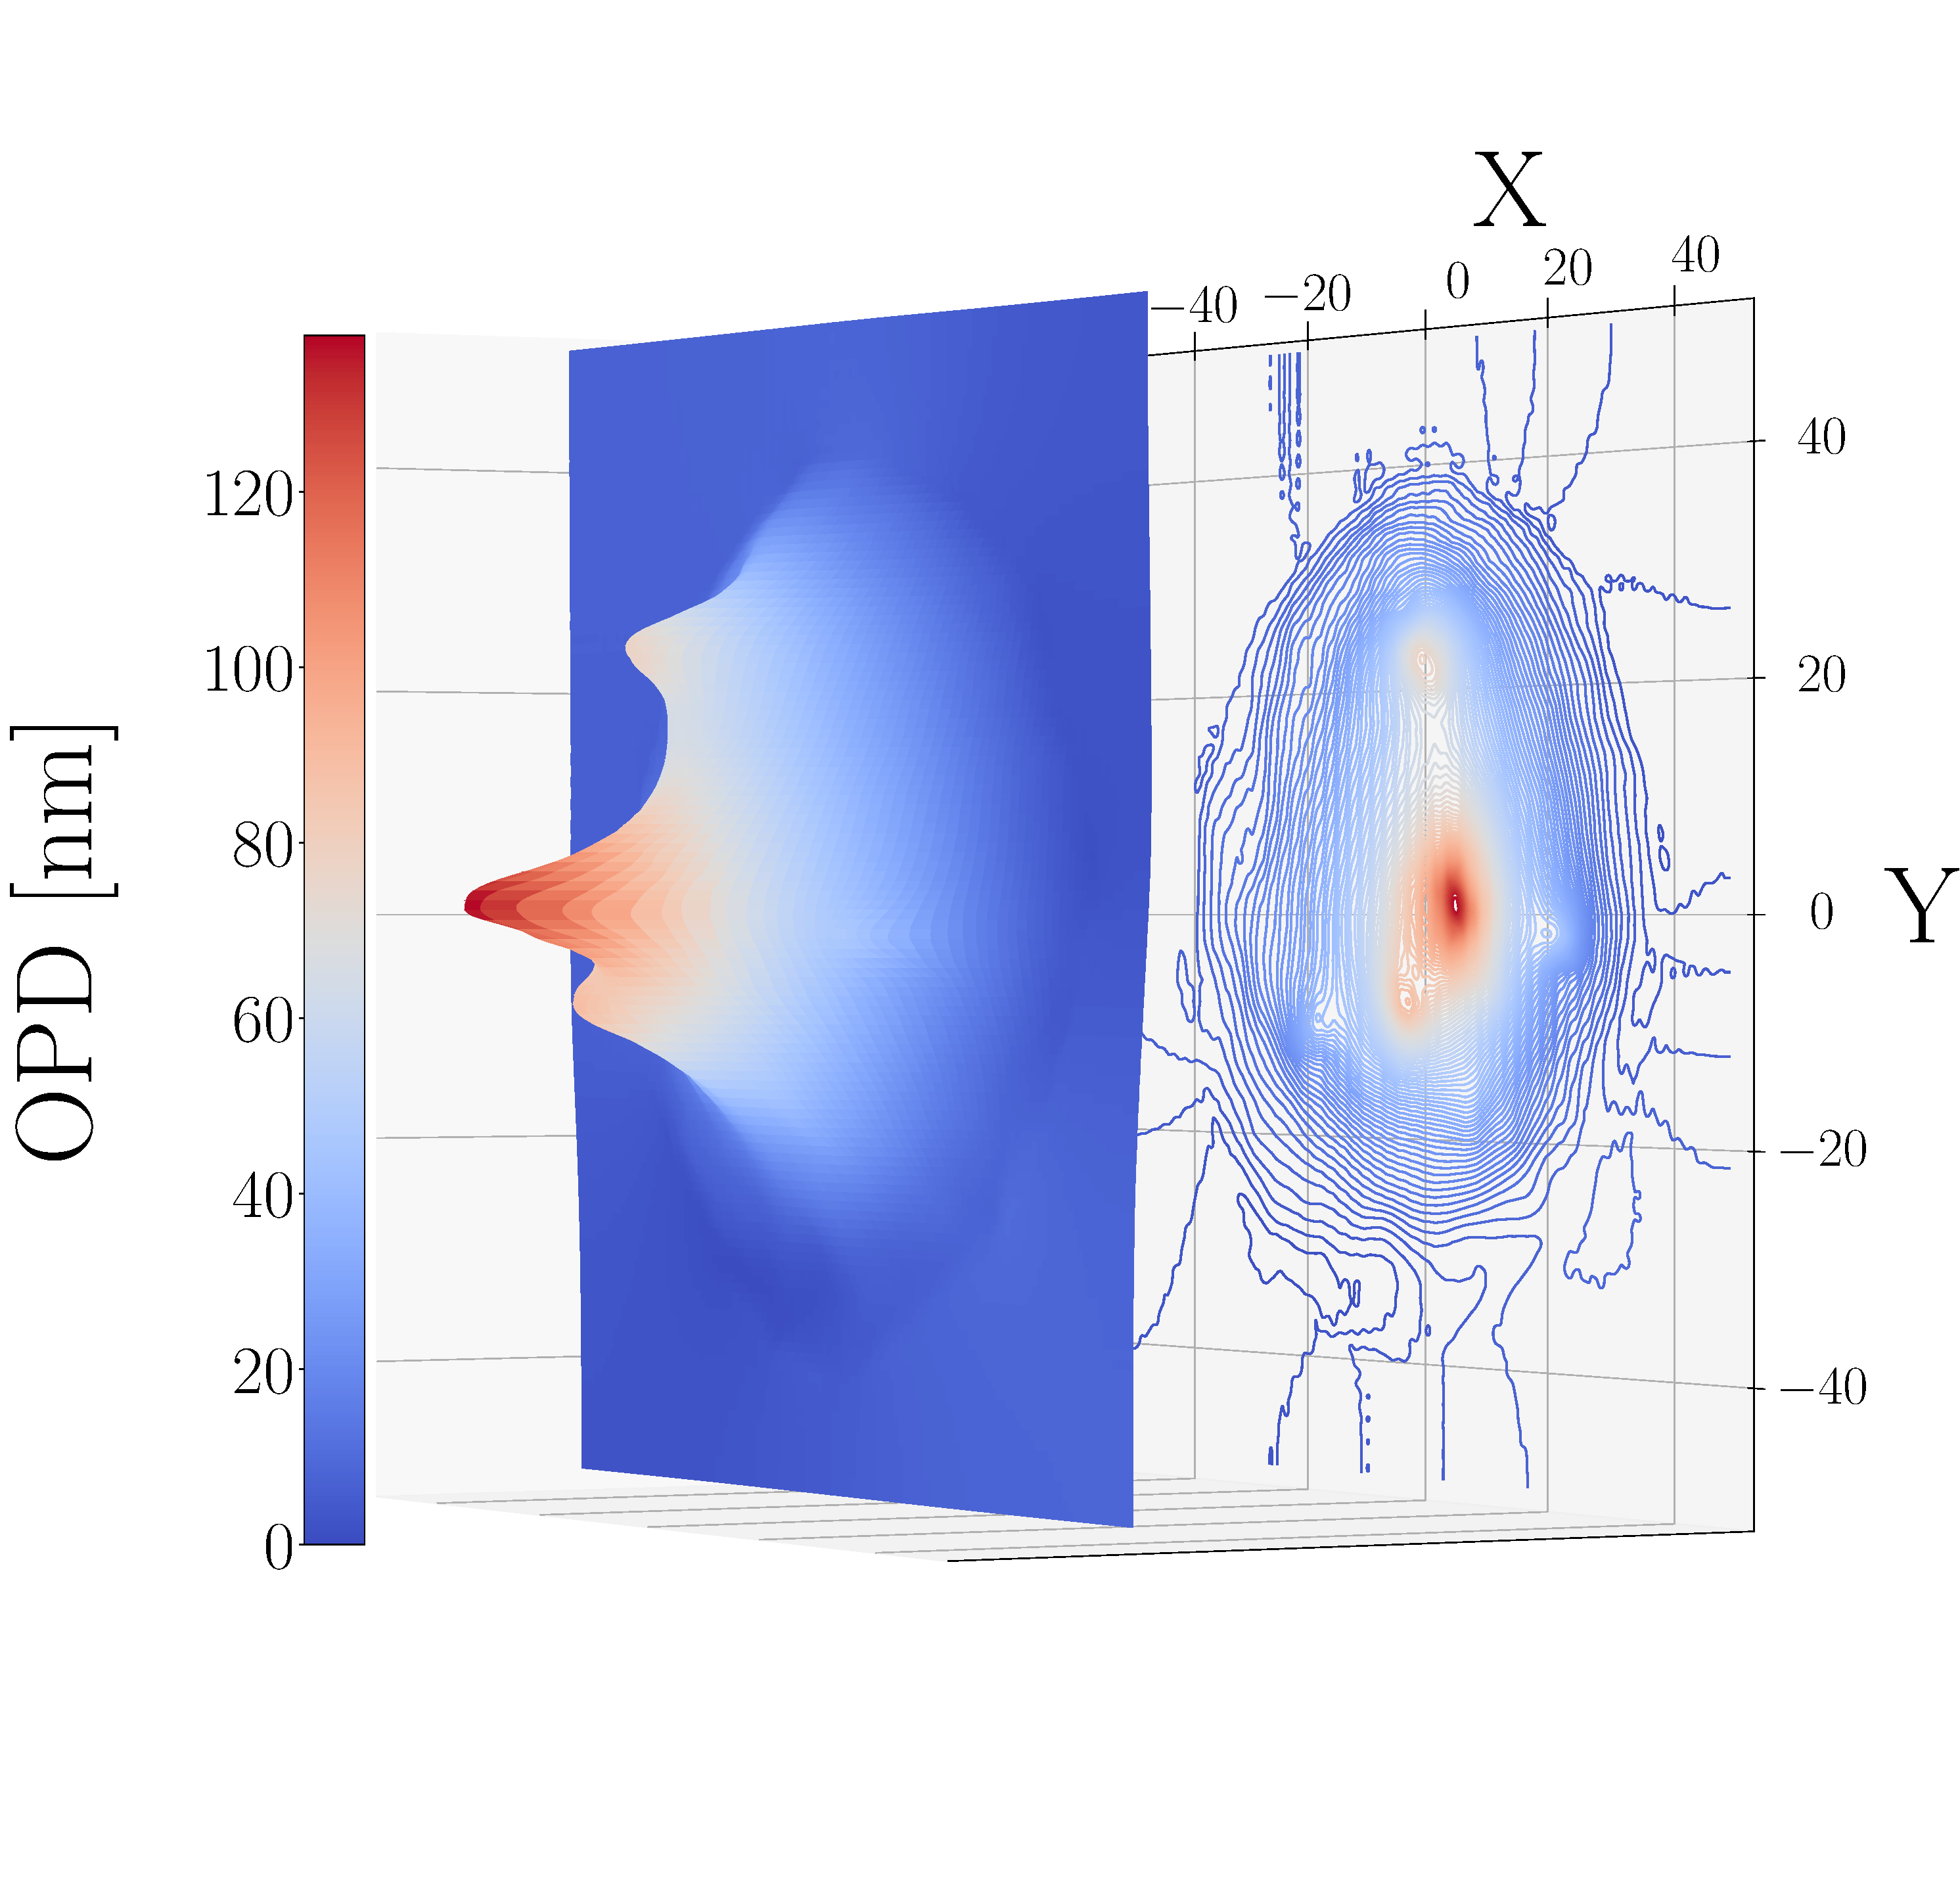
\includegraphics[width=.495\textwidth]{TCS/PA/ITMY_absorbers.pdf}
	  \phantomcaption\label{subfig:itmypajustself}
	  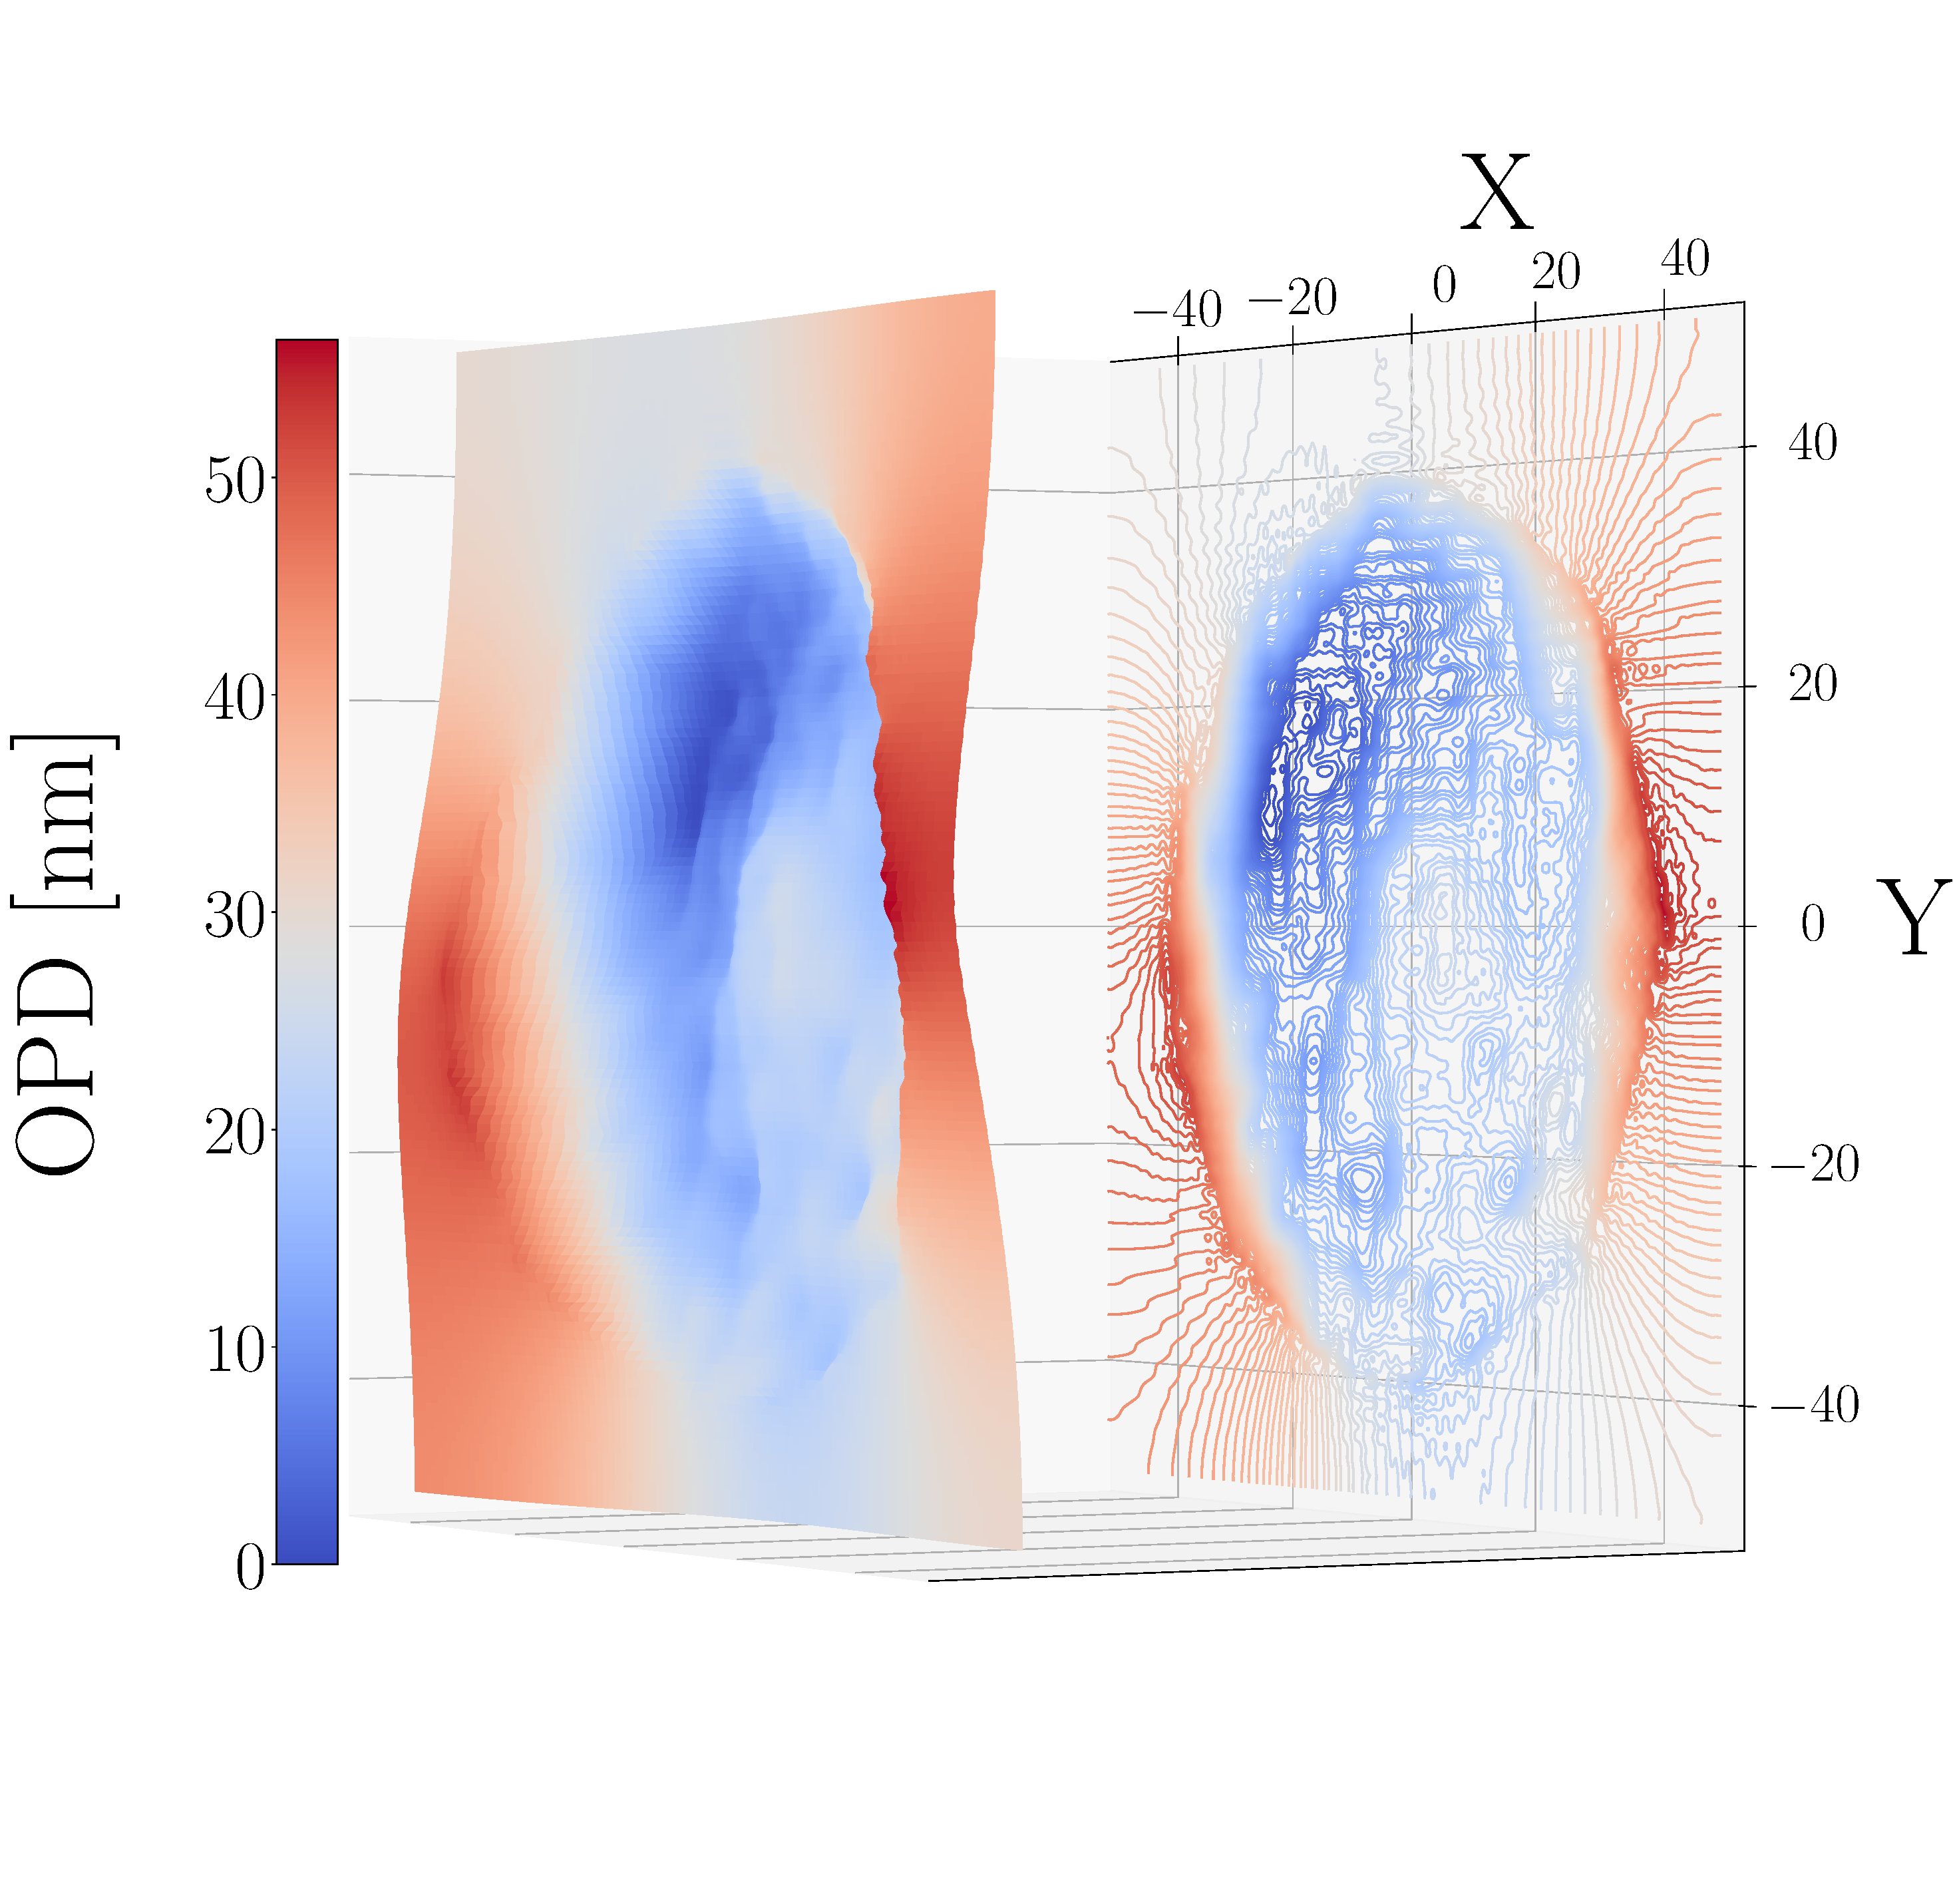
\includegraphics[width=.495\textwidth]{TCS/PA/ITMY_self.pdf}
	  \phantomcaption\label{subfig:itmypaselfplusabs}
  \end{subcaptiongroup}
  \captionsetup{subrefformat=parens}
  \hfill
  \caption{An isometric view of uniform absorption vs point absorption of LHO ITMY}
  \label{fig:ITMYpabs}
\end{figure}

\subsubsection{ETMX absorbers}
\begin{figure}[H]
  \centering
  \begin{subcaptiongroup}
	  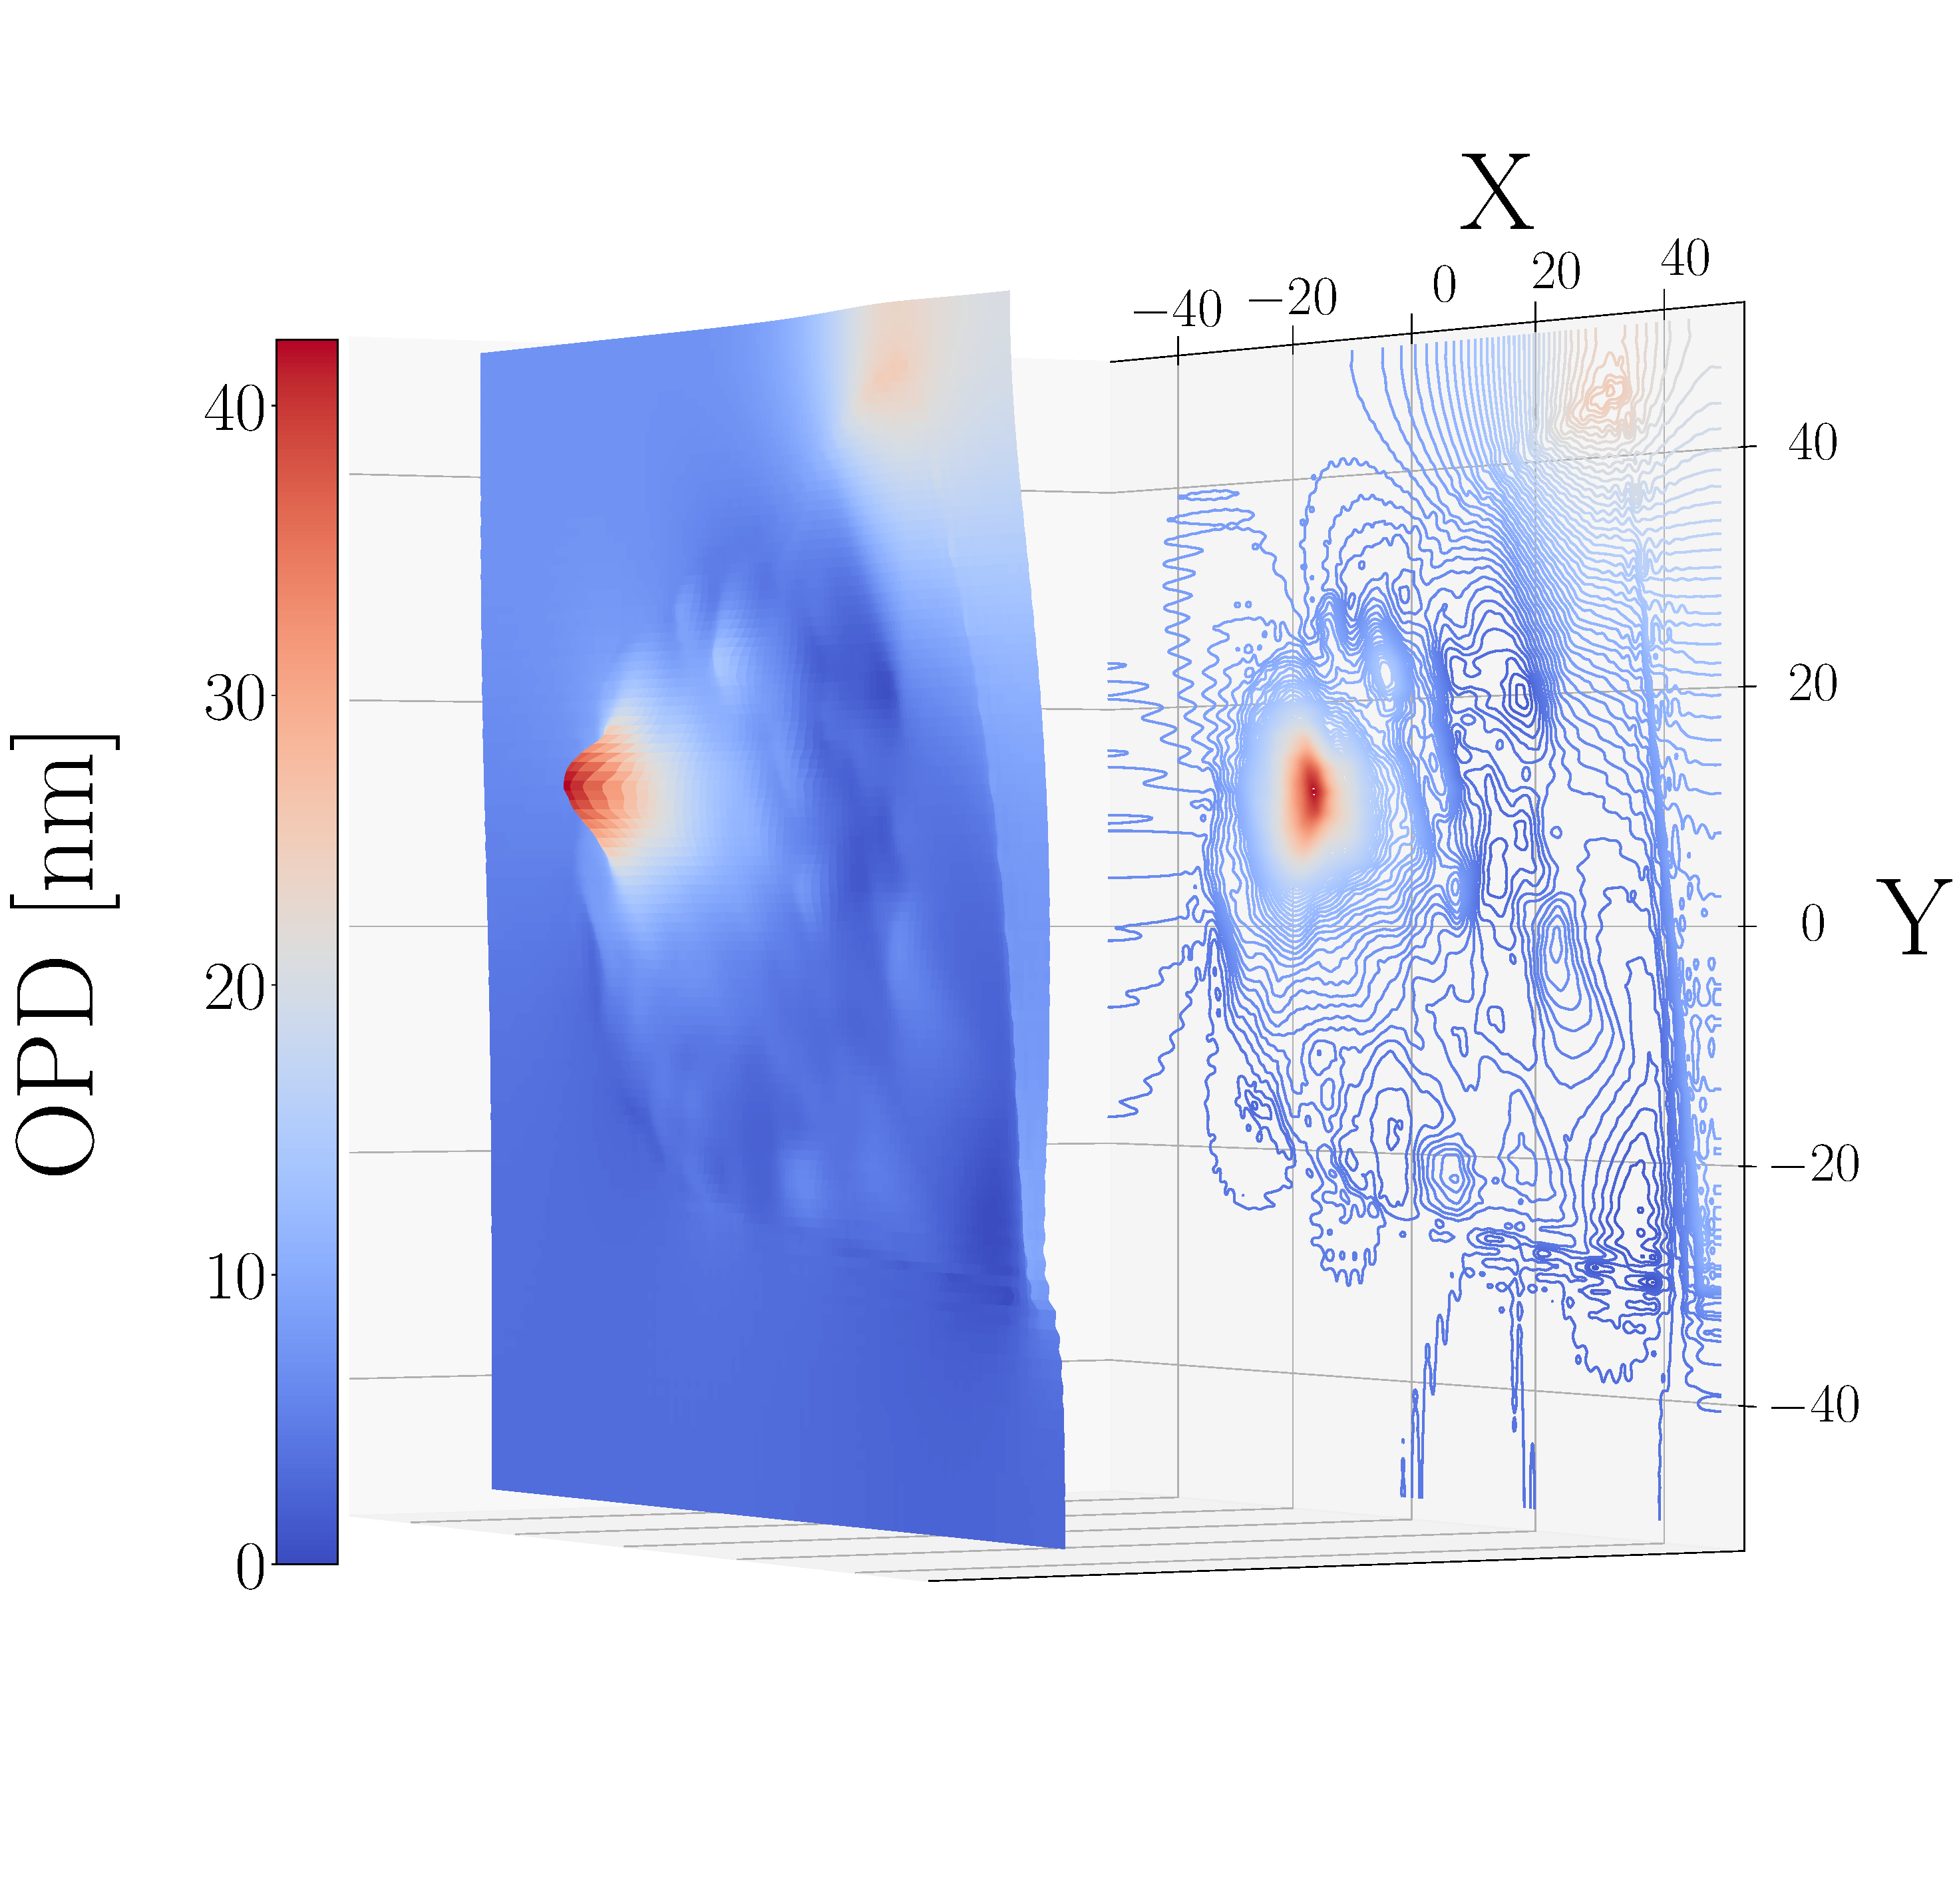
\includegraphics[width=.49\textwidth]{TCS/PA/ETMX_absorber_short_heat.pdf}
	  \phantomcaption\label{subfig:etmxpajustself}
	  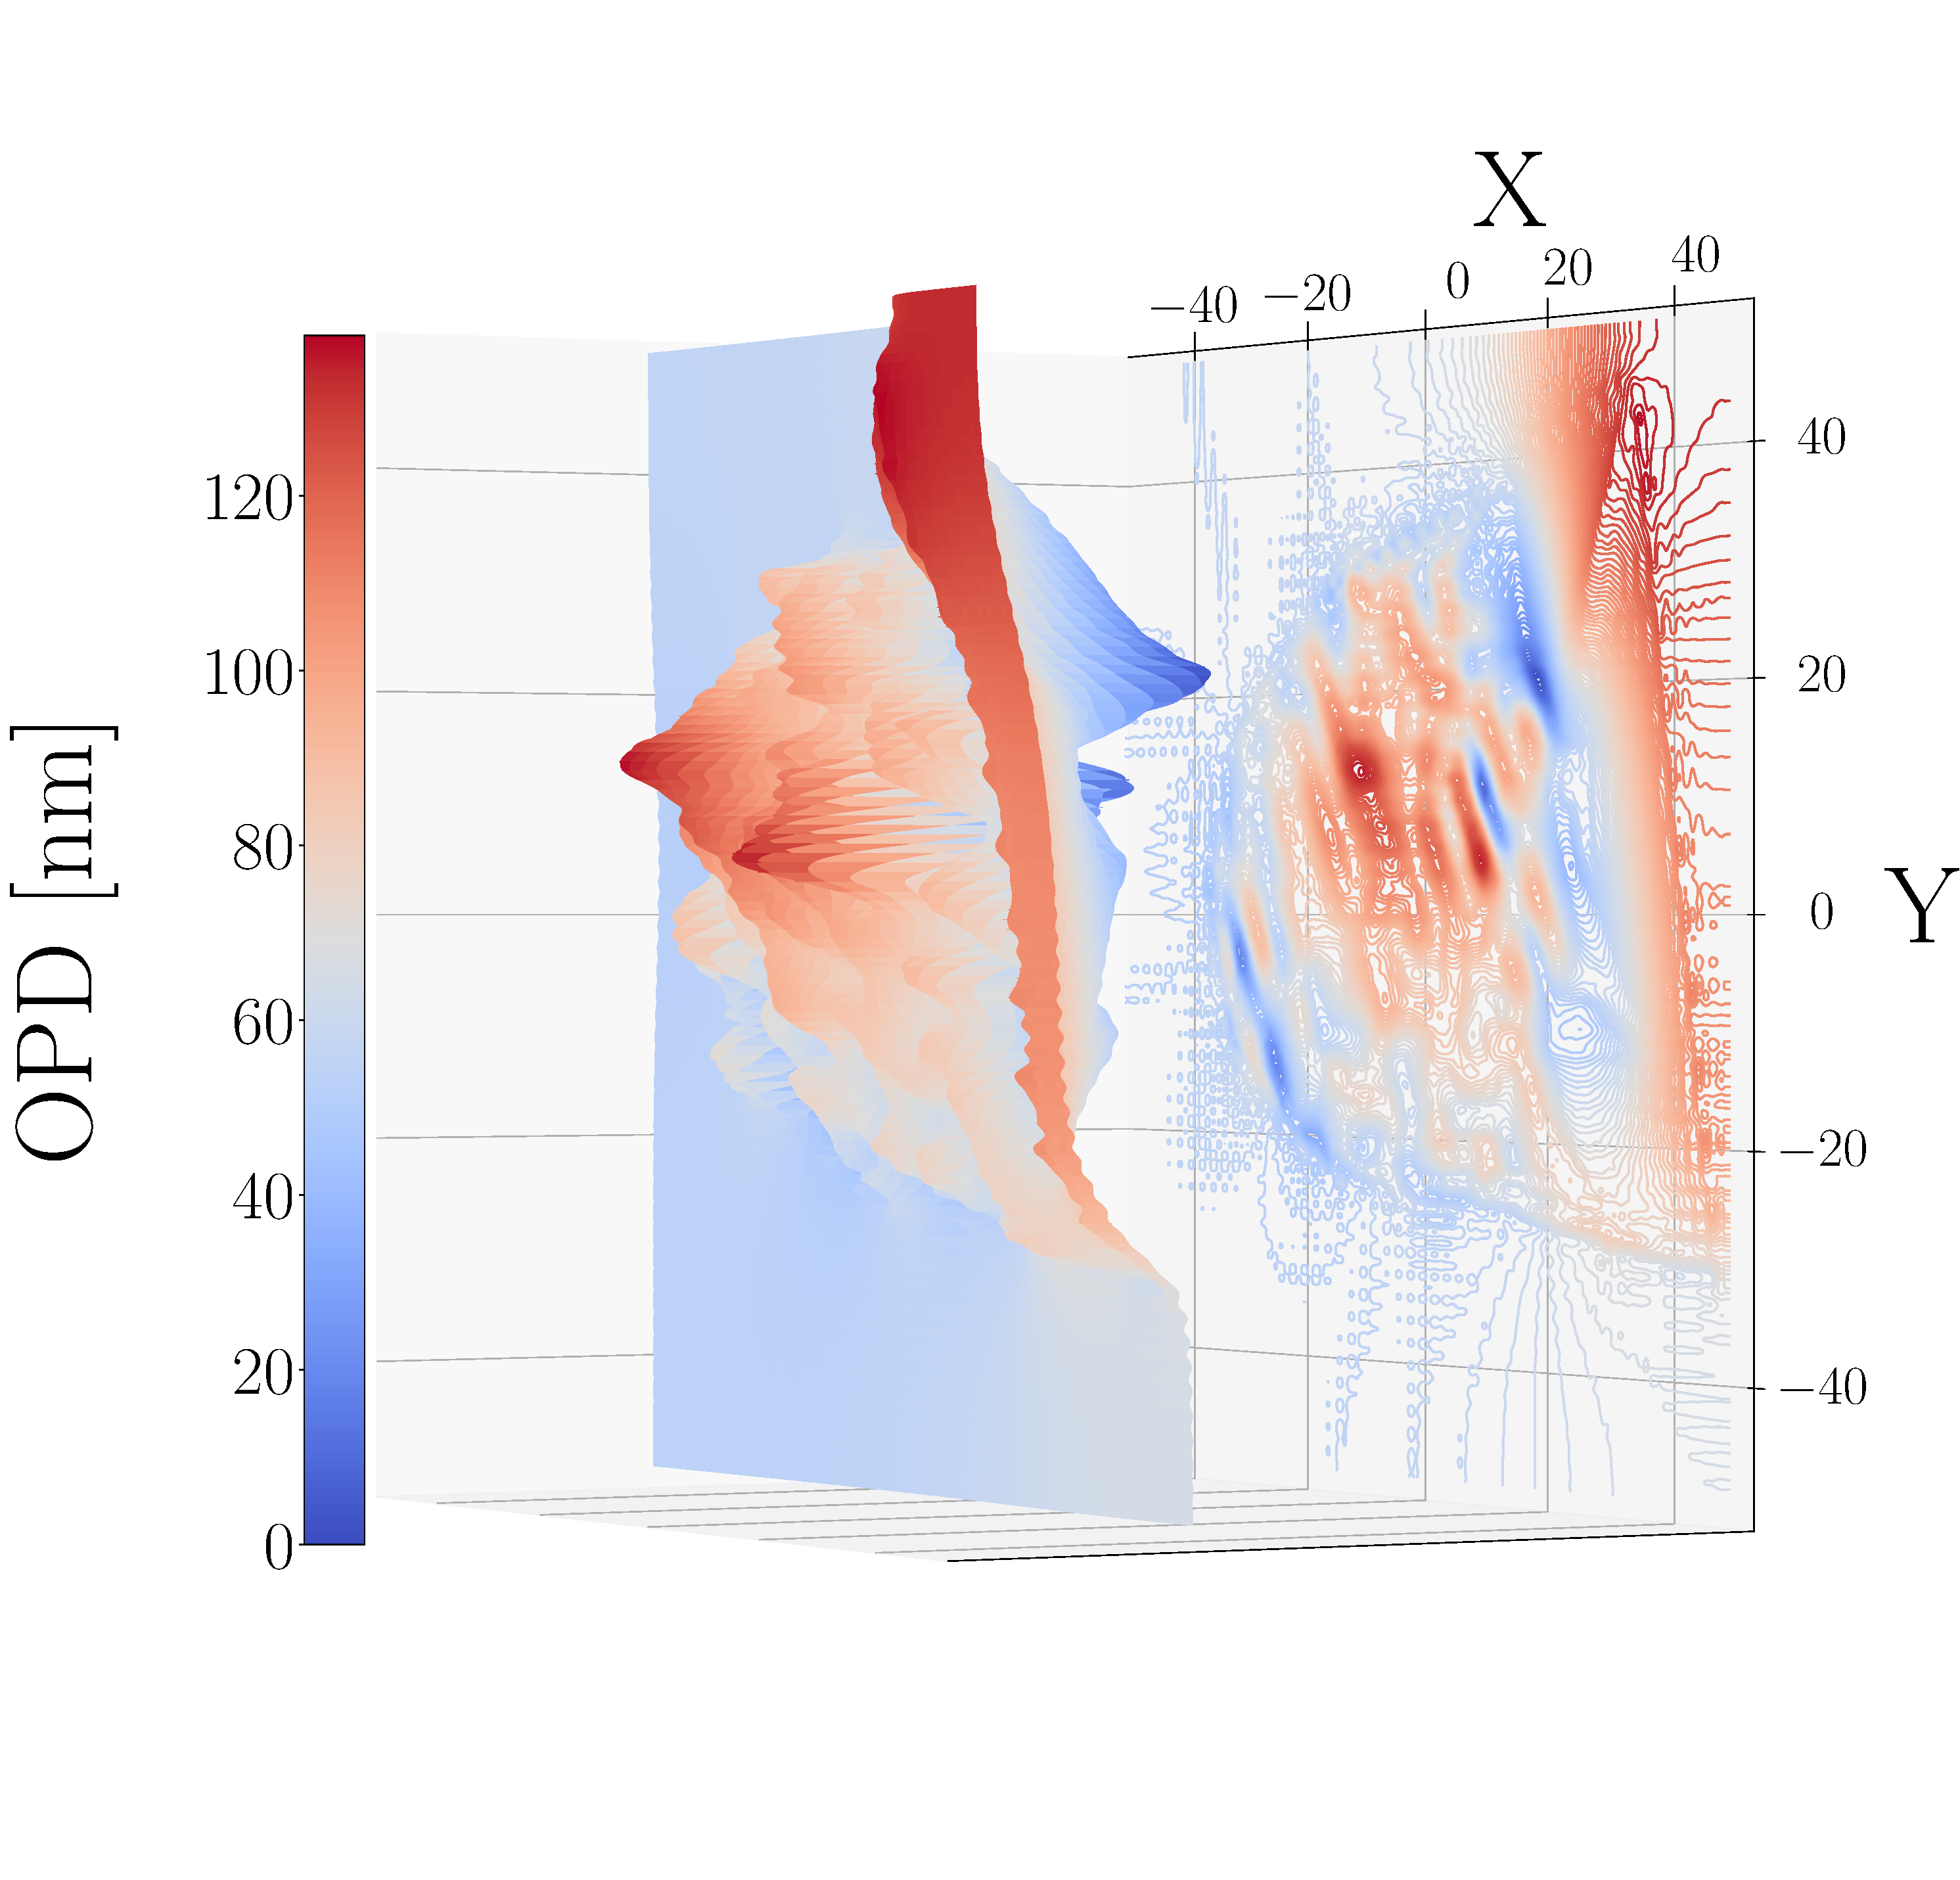
\includegraphics[width=.49\textwidth]{TCS/PA/ETMX_absorber_full_heat.pdf}
	  \phantomcaption\label{subfig:etmxpaselfplusabs}
  \end{subcaptiongroup}
  \captionsetup{subrefformat=parens}
  \hfill
  \caption{An isometric view of uniform absorption vs point absorption of LHO ETMX. The rippling / edge effects are a consequence of the Hartmann probe beam experiencing unavoidable clipping on the baffle due to misalignment of in-vaccum optics.}
  \label{fig:ETMXpabs}
\end{figure}

Impact on interferometer contrast and transmission / co-resonance of higher order modes

\subsubsection{Impacts}
A significant number of lockloss events during the comissioning period for O3A when increasing detector input power were a direct result of select optical sideband power degredation used to maintain the delicate coupled cavity configuration. And while sustaining interferometer DC readout the arm cavity would generate higher order modes sustained by Output Mode Cleaner (OMC) co-resonance; contaminating the carrier field at the output photodiode.

\paragraph{Controls schema}
\textcolor{red}{Sensor schema for interferometer control and dramatic impact to optical sidebands (higher order beat signals)}
\paragraph{Frequency noise}
\paragraph{Parasitic higher order modes}
Visible higher order modes at the anti-symmetric port \\
A significant amount of optical loss as a result of losing sideband power is reported \\
	* Lockloss caused by reduced sideband power with interferometer thermalization \\

\subsubsection{Attempted symptom reduction}
The trivial solution of reducing the test mass non-uniformity was tried but exhibited noticable limitations with the available degrees of freedom. To restore the uniformity of the test mass surface, a custom mask was constructed with the intention of imaging a negative of the optical path distortion high absorption points onto the surface with the CO2 laser combined with a static ring heater offset. 

The installation location of the mask and size was established using the relevant propogation and imaging tensors applied to the CO2 actuation field while mitigation of the aforementioned impacts provided comissioners with the notable metrics of success.

\textcolor{red}{Results}
\\
The extremely strict alignment requirement introduced difficulties while attempting to fulfill the promise of restoring uniform absorption. And although the presence of the absorber symptoms show coorelation with their prominence at high power, their collective reduction proved not to be as straightfoward~\cite{brooks:aigwd2019, buikema:2020}.
	
	* CO2 with enhanced focus on absorbers and ring heater actuation
		* Very narrow alignment requirement
		* Improvement metrics
			* Restoring sideband power	
	* Adjusting interferometer to OMC mode matching
		* Improvement metrics:
			* Reduced HOM content at detector output
			* Tracking dither line amplitudes

%\begin{figure}[H]
%\includegraphics[width=\textwidth]{figs/TCS/PA/48349_20190409201649_inital_install_CO2Ymask2_150seconds_900mW.png}
%\caption{Point absorber figure with second $\mathrm{CO_2}$ mask}
%\label{fig:RH_power}
%\end{figure}




\chapter{Electro-optic study of an  GaAs/\textbf{Al}$_{.92}$\textbf{Ga}$_{.08}$\textbf{As} coated sample}
%% Electro-optic study of AlGaAs coated mirrors

 As mentioned in Section \hyperref[sec:ligo_noise] one of the many LIGO fundamental noise sources is coating thermal noise from the $\mathrm{SiO_2}/\mathrm{TiO_2:Ta_2O_5}$ aLIGO coatings. As aLIGO approaches its designed sensitivity various coating solutions are currently proposed to mitigate thermal noise coupling into the detector output \cite{?}. With the potential to reduce coating Brownian noise by a factor of 10, $\gaas$/$\algaas$ shows much promise with next generation detectors for a potential strain reduction by a factor of 5 \cite{Cole:2013}, in comparison to the current aLIGO coatings. Though inherent material property differences of these crystalline coatings introduce new and potentially significant noise couplings; one being the linear electro-optic property of crystalline materials (dn/dE), also known as the Pockels effect \cite{abernathy_poster}. Prior to commitment of a $\gaas$/$\algaas$ coating in gravitational wave detectors, a thorough study of these notable noises is worthwhile. This section details a study of starting with a survey of the distinguishing optical and material properties of crystalline materials like $\gaas$ and $\algaas$ by reviewing: light propogation through anistropic materials, and induced optical anisotropy of zincblende materials. Immediately after, estimates of the differential phase of lightereflected from a $\gaas$/$\algaas$ coating caused by electric field noise are computed with potential impacts to current generation gravitational wave detectors. With adequate motivation, an experiment designed to measure the pockels effect from a HR $\gaas$/$\algaas$ coated ``witness" sample was constructed and the design, results are discussed.

\subsection{Anisotropic media}
Unlike with isotropic media, we cannot assume that the index of refraction of anisotropic media is the same for all chosen wave vectors. This is a direct consequence of the birefringence of anisotropic media; characterized by the dielectric, permittivity, and polarization tensors.

\subsubsection{The Dielectric tensor}
Further elaborating on the nature of a generalized dielectric tensor for any wavevector is required to proceed:
\begin{equation}\label{eq:3.11}
D_i = \varepsilon_{ij}E_j
\end{equation}
Where D is the displacement vector and E is the electric field vector and $\varepsilon$ is the dielectric tensor. The displacement vector for isotropic media is retrieved when $i = j$ and $\varepsilon_i = \varepsilon$. To further understand the nature of the dielectric tensor we assert Poynting's theorem providing an energy conservation requirement:
\begin{equation}\label{eq:3.12}
\nabla \cdot \vec{S} = \frac{dU}{dt}
\end{equation}
Where $\vec{S} = \vec{E} \times \vec{H}$ is the poynting vector and $U = \frac{1}{8 \pi} \big( \vec{E} \cdot \vec{D} + \vec{B} \cdot \vec{H} \big)$ is the electromagnetic field density. The reader is left to perform the exercise and show that in order for \ref{eq:3.12} to hold true given \ref{eq:3.11}


\begin{equation}
\varepsilon_{ij} = \varepsilon_{ji}
\end{equation}
Demonstrating that the dielectric tensor is symmetric - exhibiting only six unique terms. Diagonalizing the tensor, the presence of two unique eigenvectors and eigenvalues indicates the existance of two eigenpolarizations with paired eigenindices.
%The most general form of the energy density can be geometrically represented as ellipsoid but a coordinate transformation we can diagonalize and realize the principal axes of the dielectric allowing a simpler form of the displacement, and in turn the energy density.

\subsubsection{Monochromatic plane wave propogation}
Revisiting Maxwell's equations for simple monochromatic plane wave solution gives provides further direction on how crystalline media may effect incident light. Further elaborating, the following assumptions are made:
\begin{equation}
\vec{E} = E_o e^{(i \omega (\frac{n}{c} \vec{r}\cdot \vec{s}-t))}
\end{equation}
Where $n$ is the index of refraction, $c$ is the speed of light, $\vec{r}$ is the position vector and $\vec{s}$ is the unit wave normal.
\begin{equation}
\nabla \times \vec{H}= \frac{\partial \vec{D}}{\partial t}
\end{equation}
Where $\vec{H}$ is the magnetic field assuming the permeability $\mu$, and the generalized displacement vector $\vec{D}$ and electric field vector $\vec{E}$.
\begin{equation}
\nabla \times \vec{E} = -\mu \vec{H}
\end{equation}
Reducing to only the displacement and electric fields:
\begin{equation}\label{eq:3.17}
\vec{D} = \frac{n^2}{\mu}[\vec{E}-\vec{s}(\vec{s}\cdot \vec{E})]
\end{equation}
Maxwell's equations show that the electric field is not necessarily parallel to the displacement field and in most materials with non-zero polarizability tensors and dielectric tensors, it is not. But as specified above, the displacement vector, Electric field and unit wave normal are co-planar while remaining orthogonal to $\vec{H}$. Assuming we are operating within a coordinate system aligned with the principal dielectric axes, we substitute \ref{eq:3.11} into \ref{eq:3.17}:
\begin{equation}\label{eq:3.18}
E_i = \frac{n^2 s_i (\vec{E}\cdot\vec{s})}{n^2 - \mu \varepsilon_i}
\end{equation}

From here it can be shown that for a general plane wave there exist two unique refractive index solutions within the constructed dielectric. Though using this result to show this requires revisiting geometrical conditions that are best visualized using a method introduced in the next section. \textcolor{red}{For a more rigorous proof, see Appendix H in} \cite{nye}

\subsubsection{Indicatrix}\label{sec:indicatrix}
Acquiring solutions of the two indices along with the corresponding directions of propogation in the crystal for a general plane wave with unit wave vector $\vec{s}$ can be done via a conveniant geometrical construction. The construction begins by considering a constant electric energy density ($U_e$) surface in the $\vec{D}$ space; an ellipsoid is formed:

\begin{equation}\label{eq:lagr1}
\frac{D_x}{\varepsilon_x} + \frac{D_y}{\varepsilon_y} + \frac{D_z}{\varepsilon_z} = 2 U_e \varepsilon_o
\end{equation}
With redefined coordinates $(\vec{D}/\sqrt{2 U_e \varepsilon_o}) \rightarrow \vec{r}$ and setting $\varepsilon_i = n^2_i$:
\begin{equation}
\frac{x^2}{n_x^2} + \frac{y^2}{n_y^2} + \frac{z^2}{n_z^2} = 1
\end{equation}
This equation for the ellipsoid is known as the indicatrix. Given the co-planar solution demonstrated in the last section, we can impose the normal of the plane $\vec{r} \cdot \vec{s} = 0$:

\begin{equation}\label{eq:lagr2}
\vec{r} \cdot \vec{s} = x s_x + y s_y + z s_z = 0
\end{equation}
Equations \ref{eq:lagr1} and \ref{eq:lagr2} both contribute constraints to the method of finding extrema using Lagrange multipliers for the function:
\begin{equation}
r^2 = x^2 + y^2 + z^2
\end{equation}
The Lagrangian ($\mathcal{L}$) with the introduced multiplers ($\lambda_1$, $\lambda_2$) then becomes:
\begin{equation}
\mathcal{L}(\textcolor{red}{\vec{r},\vec{s}},\lambda_1, \lambda_2) =
x^2 + y^2 + z^2 + \lambda_1 (xs_x + ys_y + zs_z) + \lambda_2 \bigg( \frac{x^2}{\varepsilon_x} + \frac{y^2}{\varepsilon_y} + \frac{z^2}{\varepsilon_z} - 1 \bigg)
\end{equation}
With the generated system of equations from the Lagrange multipler method ($\partial F_i/ \partial x_i = 0$, and $\partial F_j/ \partial \lambda_j$) where index $i =x,y,z$ and $j = 1,2$ we obtain a system of 3 equations:
\begin{equation}
i \bigg(1-\frac{r^2}{\varepsilon_{i}} \bigg) + s_{i} \bigg(\frac{x s_x}{\varepsilon_x} + \frac{y s_y}{\varepsilon_y} + \frac{z s_z}{\varepsilon_z} \bigg) = 0
\end{equation}
The result is verified when substituting $r \rightarrow \frac{\vec{D}}{\sqrt{\vec{E} \cdot \vec{D} \varepsilon_o}}$ back which recovers \ref{eq:3.18}.
\\

\begin{figure}[H]
\begin{center}
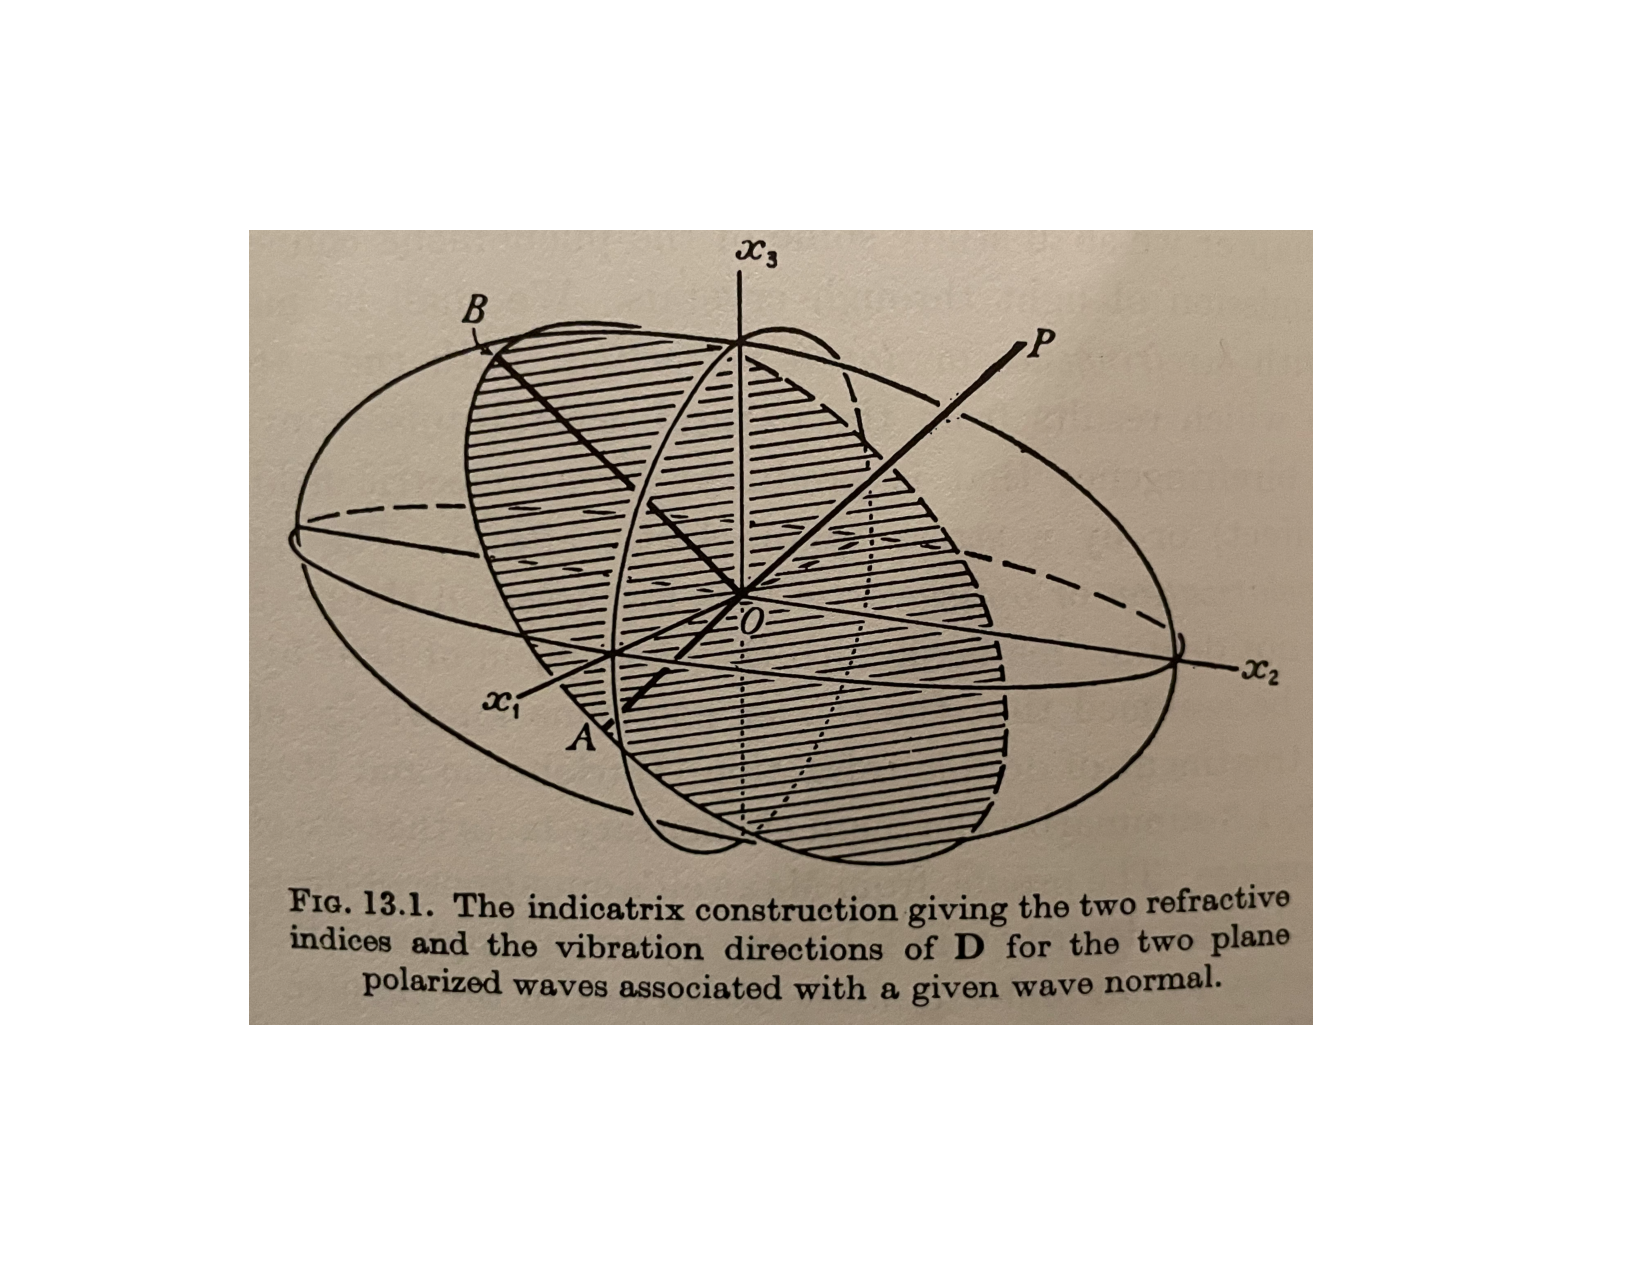
\includegraphics[width=75mm]{figs/ALGAAS/indicatrix_nye.pdf}
\end{center}
\caption{General ellipsoid indicatrix with a general propogation direction (Using Nye's figure as placeholder as of now)}
\label{fig:general_indicatrix}
\end{figure}

\subsection{$\gaas$ and $\algaas$ crystal classification}
The space group of $\gaas$ as well as $\algaas$ are within the $F\bar{4}3m$ space group. Crystals of this particular space group are commonly known as zincblende crystals; a common crystal configuration named after zinc sulfide (ZnS). Cubic crystals by their crystallographic structure display optically isotropic characteristics when  stress free and no DC and/or slowly varying electric fields are present.
\satoshi{Is this true?} \textcolor{blue}{Yes. Though the birefringence seen from HR $\gaas$ coatings is said to be due to an ``intrinsic stress" in the high and low index layers. (What is breaking the symmetry to cause this? Heteroepitaxy? Annealing? Defects? Is this birefringence the same for all samples?) I think a dedicated high precision birefringence measurement on multiple samples would be cool.}

\begin{figure}[H]
\begin{center}
\includegraphics[width=.85\textwidth]{figs/ALGAAS/gaas_unit_cell_mi.pdf}
\caption{The unit cell of gallium arsenide (GaAs) with associated miller indices as coordinate axes}
\end{center}
\label{fig:gaas_uc}
\end{figure}

\textcolor{red}{Mention the difference in lattice cell constant between $\gaas$ and $\algaas$?}

\subsection{Induced anisotropy in zincblende crystals}
Zincblende structures, like the crystalline materials in question can exhibit birefringent properties when under the influence of two factors: stress in the material, and present within DC electric fields. These two properties of crystalline materials are known as the photoelastic and electro-optic effects respectively.

\subsubsection{The (linear) electro-optic (Pockel's) effect}

For non-centrosymmetric crystalline media there exists a non-zero rank 2, $6 \times 3$ tensor ($r_{ij}$) connecting a low-frequency \footnote{"low frequency" meaning orders of magnitude smaller than an optical field it effects} electric field $\vec{E}(f) = [E_x(f), E_y(f), E_z(f)]$ directly to the \hyperref[sec:indicatrix]{indicatrix} ~\cite{yariv,nye}:
\begin{equation}
  \left[ {\begin{array}{c}
   \big( \frac{1}{\Delta n ^2 } \big)_1 \\
   \big( \frac{1}{\Delta n ^2 } \big)_2 \\
   \big( \frac{1}{\Delta n ^2 } \big)_3 \\
   \big( \frac{1}{\Delta n ^2 } \big)_4 \\
   \big( \frac{1}{\Delta n ^2 } \big)_5 \\
   \big( \frac{1}{\Delta n ^2 } \big)_6 \\
  \end{array} } \right]
  =
%
 \left[ {\begin{array}{ccc}
   r_{11} & r_{12} & r_{13}\\
   r_{21} & r_{22} & r_{23}\\
   r_{31} & r_{32} & r_{33}\\
   r_{41} & r_{42} & r_{43}\\
   r_{51} & r_{52} & r_{53}\\
   r_{61} & r_{62} & r_{63}\\
  \end{array}} \right]
 %
 \left[{\begin{array}{c}
   E_x (f)\\
   E_y (f)\\
   E_z (f)\\
 \end{array}} \right]
\end{equation}

\noindent The $i$ index runs over the terms in the indicatix equation:
\begin{equation}
\bigg(\frac{1}{\Delta n_x^2} \bigg) x^2\ + \bigg(\frac{1}{\Delta n_y^2} \bigg) y^2 + \bigg(\frac{1}{\Delta n_z^2} \bigg) z^2 + 2 \bigg(\frac{1}{\Delta n_{xz}} \bigg)xz + 2 \bigg(\frac{1}{\Delta n_{yz}} \bigg)yz + 2 \bigg(\frac{1}{\Delta n_{xy}} \bigg)xy = 1
\end{equation}

\noindent \textcolor{red}{Detail on some prior knowledge of $f \leq f_\mathrm{max}$? (Pockels cell specs?)}


\subsubsection{$r_{ij}$ for zincblende crystals ($r_{\bar{4}3m, ij}$)}

The form of the electro-optic tensor for zincblende crystals (including $\gaas$ and $\algaas$) reduces such that $r_{ij} = r_{41} = r_{52} = r_{62} \neq 0$ with all other terms being zero:

\begin{equation}
r_{\bar{4}3m,ij} =
 \left[ {\begin{array}{ccc}
  0 & 0 & 0\\
  0 & 0 & 0\\
  0 & 0 & 0\\
  r_{41} & 0 & 0\\
  0 & r_{52} & 0\\
  0 & 0 & r_{63}\\
 \end{array}} \right]
\end{equation}

\noindent Where also $r_{41} = r_{52} = r_{63}$

\subsubsection{New principal (electro-optic) dielectric axis for zincblende structures}

In general the principle dielectric axes of the new ellipsoid do \textbf{not} coincide with the axes of the ellipsoid of the unperturbed crystal. The form of the index ellipsoid for a zincblende crystalline material accounting for the electro-optic tensor and some generalized DC electric field $\vec{E}$ expressed in terms of the crystallographic axes is given by:
\begin{equation}\label{eq:zindicatrix}
\bigg(\frac{1}{n_o^2} \bigg) x^2\ + \bigg(\frac{1}{n_o^2} \bigg) y^2 + \bigg(\frac{1}{n_o^2} \bigg) z^2  + 2r_{41} E_{[100]} yz + 2r_{41} E_{[010]} xz + 2r_{41}E_{[001]} xy= 1
\end{equation}

\noindent Where we have set $n_x = n_y = n_z = n_o$ for zincblende structures.

\noindent The two principal axes are given by the eigenvectors of the the matrix given from the equation above:

\begin{equation}
 \left[ {\begin{array}{ccc}
   \big( \frac{1}{n_o ^2} \big)& r_{41}E_{[001]} & r_{41} E_{[010]}\\
   r_{41}E_{[001]} & \big( \frac{1}{n_o ^2} \big) &  E_{[100]}\\
   r_{41} E_{[010]} & r_{41} E_{[100]} & \big( \frac{1}{n_o ^2} \big)\\
  \end{array}} \right]
\end{equation}

\subsubsection{The photoelastic effect}

When a general strains $S_{kl}(r) = \frac{1}{2} \bigg[ \frac{\partial u_k (r)}{\partial x_i} + \frac{\partial u_i (r)}{\partial x_k} \bigg]$ are applied to a material, the photoelastic tensor $p_{idkl}$ relates to the indicatrix by the following relation:

\begin{equation}
 \bigg( \frac{1}{\Delta n^2} \bigg)_{id} = p_{idkl} S_{kl}
\end{equation}

\textcolor{red}{Supplementary comment to the measured birefringence from the mentioned intrinsic strain of the high and low index layers}

\subsubsection{The generalized indicatrix}


\begin{equation}
\bigg( \frac{1}{\Delta n^2} \bigg)_{ij} = r_ijE_j + p_{ijkl} S_{kl}
\end{equation}

\textcolor{red}{Need to fix these indices}
\\
\textcolor{red}{New principal dielectric axes for zincblende structures (zinblende photoelastic tensor, zincblende electro-optic tensor)}

\subsection{Electro-optic modulation}\label{sec:EOM}
A common application of this effect is phase modulation onto a optical carrier field. Electro-optic modulators or Pockel cells accomplish this by sandwiching two capacitor plates around crystal with a single electrical input port designed to take in a frequency ($\Omega$) within a specified modulation bandwidth. When the field amplitude across the crystal is driven by a voltage controlled oscillation, we exiperience a change in the electro-optic tensor. The voltage amplitude of the signal input is proportional to the strength of the phase modulation on the optical carrier field of frequency ($\omega$) and is commonly quantified in terms of a modulation index ($\beta$).

\begin{figure*}[!h]
     \begin{subfigure}{\includegraphics[width=.5\textwidth]{figs/ALGAAS/temp/pockels_cell_l.pdf}}
     \end{subfigure}
     \hfill
     \begin{subfigure}{\includegraphics[width=.5\textwidth]{figs/ALGAAS/temp/pockels_cell_t.pdf}}
     \end{subfigure}
    \caption{\textcolor{red}{PENDING UPDATES currently borrowed image from rp photonics} Longitudinal and Transverse Pockels cells}
    \label{fig:lpc_and_tpc}
\end{figure*}



\textcolor{red}{Consider specific crystal that gives us our $\beta \mathrm{sin}(\Omega t)$}


\begin{equation}\label{eq:inp_EOM}
E_\mathrm{inp} = E_o e^{i \omega t + \beta \mathrm{sin}( \Omega t)}
\end{equation}

\textcolor{red}{This construction resembles that of the electrostatic optical mount used to drive a longitudinal electric field}

\subsection{Optical anisotropy of a HR $\gaas$ / $\algaas$ stack}
Our interests primarily lie with the study of birefringent properties of a candidate highly reflective $\gaas$/$\algaas$ mirrorstack. This section is intended to provide a comprehensive review by: 1) making considerations of crystal coordinates when asserting an optical axis on a highly reflective crystalline stack manufactured by Thorlabs, 2) citing coating parameters and observed intrinsic birefringence from the highly reflective coating stack in question, 3) analyzing differential linear electro-optic effect on the phase of a reflected beam, and 4) estimating the the differential phase noise in LIGO based on calibrated electric field measurements.

\begin{figure*}[!h]
    \begin{subfigure}{\includegraphics[width=.5\textwidth]{figs/ALGAAS/coating_orientation_normal.pdf}}
    \end{subfigure}
    \hfill
    \begin{subfigure}{\includegraphics[width=.5\textwidth]{figs/ALGAAS/coating_orientation_isometric.pdf}}
    \end{subfigure}
\caption{The beam propogation axis ($\vec{S}$, $[-100]$) with respect to the AlGaAs/GaAs crystal axes. The axis formed by the [100] plane normal is parallel with the beam axis (z-axis) and the polarizations of incident and reflected beam oscillate along vectors within the plane formed by the normal of that axis. The AlGaAs coating is grown with a flat indicating a line within the [0-11] plane; where the plane normal points towards the sample center.}
\label{fig:algaas_coords}
\end{figure*}

\subsubsection{Miller indices for highly reflective coatings $\gaas$/$\algaas$ coatings}

Up until this point we have discussed three different coordinate axes: the crystal axis (indicated by Miller index plane normals), the principal dielectric axis (coordinates based in diagonalization of the indicatrix), and an optical axis (when considering a desired (laser) light propogation). We assert the beam axis \cite{fig:algaas_coords} with linearly p-polarized light.

\subsubsection{Electro-optic coupling to the reflected phase of a HR mirror coating}
With our coordinate considerations and established beam axis, it is now worth considering the influence of an isotropic white noise field ($E_n = [E_{nx},E_{ny},E_{nz}]$):

\begin{equation}
 \left[ {\begin{array}{ccc}
   \big( \frac{1}{n_o ^2} \big)& r_{41}E_{ny} & r_{41} E_{nx}\\
   r_{41}E_{ny} & \big( \frac{1}{n_o ^2} \big) & r_{41} E_{nz}\\
   r_{41} E_{nx} & r_{41} E_{ny} & \big( \frac{1}{n_o ^2} \big)\\
  \end{array}} \right]
\end{equation}

Assuming $E_n$ is small, the indicatrix change of $E_{nx}$ and $E_{ny}$ relative to $E_{nz}$ (as seen by the beam polarization) will be small ($r_{41}E_{n(x/y)} \ll r_{41}E_{nz}$). After diagonalizing with relevant terms \footnote{Note that the form of the tensor is still in the crystal coordinates but the $E_n$ terms are placed in the tensor such that their directions align with beam axis coordinates.} in the tensor, we are left with the following eigenindices:

\begin{equation}
\begin{aligned}
n_x' & = n_o - r_{41}E_{nz} \\
n_y' & = n_o + r_{41}E_{nz}
\end{aligned}
\end{equation}

%\textcolor{red}{How the modulation of the phase of the carrier field is dependent on the orientation of its wave vector with respect to the crystal structure, the modulating electric field direction and strength, (other items to discuss in terms of introducing the effect)}
For GaAs @ $10.6\mu$ $r_{41} = 1.6 \times 10^{-12}$ [m/V]
\\
Adachi estimate for $\mathrm{Al_{x}Ga_{1-x}As}$?
\\
\textcolor{red}{Relevant eigenpolarizations, non-optical field $E_y = E_z = 0$?}
\\
\textcolor{red}{Figure: Transformed indicatrix (Before and after $E_x$)}
\\
\textcolor{red}{Figure: Ellipse cross section. New eigenpolarizations and corresponding indices and their influence on incident field (Marty's result)}
\\
Assuming we are operating in a coordinate system suggested in \hyperref[fig:algaas_coords]{Figure 3.4}, which plane is impacted by some $E_\mathrm{noise}$? Revisiting the \hyperref[eq:zindicatrix]{indicatrix} we can see that for even non-zero z and y components that the only coupling to the input beam polarization is the index along the cross coupled zy axis through $E_z$ is that of the $E_x$ term. This gives us the ability to easily diagonalize the indicatrix tensor by setting the non-relevant field terms to zero.
Fejer and Bonilla take an analytical approximation approach when finding the impact of the electric field to the change in phase of the light through a crystalline anisotropic thin film ($\lambda/4$) stack \cite{bonilla_fejer}.

\begin{equation}
\hat{\phi}' = \frac{\pi n_1 z}{1-z^2}(z^{2N} -1) \frac{z^{2N} \frac{(n_f)^2}{n_2 n_3}(n_2 \kappa_{\gamma 2} + n_3\kappa_{\gamma 3}) - (n_2 \kappa_{\gamma 3} + n_3\kappa_{\gamma 3})}{(n_1)^2 -(n_f)^2 z^{4N}}
\end{equation}

with $z = \frac{n_2}{n_3}$
and
$
\kappa_{\gamma j} = \frac{d}{d \gamma} \mathrm{log}(n_j h_j)|_{\gamma =\gamma_{O}} \bigg(\frac{\hat{n}_j'}{\hat{n}_j} +\frac{\hat{h}_j'}{\hat{h}_j} \bigg)
$

With $\kappa$ being a scalar parameter.

\textcolor{red}{FIGURE: Cross sectional view of multilayer coating}

\subsubsection{Numerical estimate}

In the appendix of \cite{ballmer2015} Ballmer constructs a coating layer transfer function for a given coating layer k with index $n_k$, and thickness $d_k$, defining right and left propogating modes $\Psi^{R,L}$ repsectively:

\begin{equation}
  \left[ {\begin{array}{c}
   \Psi^\mathrm{R} \\
   \Psi^\mathrm{L} \\
  \end{array} } \right]_{k+1}
  =
%
Q_k D_k
%
 \left[{\begin{array}{c}
   \Psi^\mathrm{R} \\
   \Psi^\mathrm{L} \\
 \end{array}} \right]
\end{equation}

\noindent $D_k$ applies the phase ($\phi_k = 4\pi n_k d_k /\lambda_0$) from a given coating layer, and $Q_k$ applies the transfer function between high-low/low-high index layers transition:

\begin{equation}
Q_k = \frac{1}{2n_{k+1}}
\left[ {\begin{array}{cc}
  n_{k+1} + n_k & n_{k+1} - n_k\\
 n_{k+1} - n_k & n_{k+1} + n_k\\
\end{array} } \right]
\end{equation}

\begin{equation}
D_k =
\left[ {\begin{array}{cc}
  e^{-i \phi_k / 2}& 0\\
 0 & e^{i \phi_k / 2}\\
\end{array} } \right]
\end{equation}
Defining a HR coating stack, the total transfer matrix from vaccum $Q_0$ to the $N$th coating layer is:
\begin{equation}
M = Q_N D_N ...Q_kD_k...Q_1D_1Q_0
\end{equation}
The impact of a differential electric noise field ($E$) on $M$ due to the electro-optic effect on the kth layer, we use the chain rule:


The coating to be studied consists 36 $\lambda$/4  thick layers of $\gaas$ interspersed with 35 layers of $\lambda$/4 thick $\algaas$.   $\gaas$ forms the top and bottom layer to prevent oxygen absorption from the AlGaAs layer. The $\gaas$ layers have an index of $n_{\gaas} = 3.480$ and a thickness of $\Delta d_{\gaas} = 76.43$ nm while the low index $\algaas$ layers are $n_{\algaas} = 2.977$ with thickness $\Delta d_{\algaas} = 89.35$ nm. With the cosntructed matrices, we apply these parameters and compute a differential phase of:

%High Index:  GaAs, n=3.480, layer thickness is 76.43 nm
%Low Index:  $ \mathrm{Al}_{0.92} \mathrm{Ga}_{0.08} \mathrm{As} $, n=2.977, layer thickness is 89.35 nm
%\textcolor{red}{Info from Steve. Written source?}


\subsection{Measured birefringence from HR $\gaas$/$\algaas$ mirrors}
There seems to be different accounts of a measured birefringence from HR $\gaas$ / $\algaas$ (\href{https://dcc.ligo.org/DocDB/0181/G2200386/001/G2200386.pdf}{Satoshi}, \href{https://nodus.ligo.caltech.edu:8081/CTN/1474}{CTN}, \href{https://dcc.ligo.org/DocDB/0181/G2200559/001/G2200559-v1%20-%20polarization.pdf}{Aidan})
\\
\textcolor{red}{Is the measured birefringence static? (Layer bonding method might introduce something?)}
\\
\textcolor{red}{Does it change from different mounting methods? (Photoelastic) (order of magnitude estimate)}
%\\
%\textcolor{red}{Electro-optic ruled out based on field measurements and relative coupling factor.}
\\
\textcolor{red}{Measurement precision of the coating birefringence? Cavity length, Polarization drifts, etc.}
\\
The measured birefringence is estimated to be caused by an intrinsic strain between the epitaxial layers of $\gaas$/$\algaas$. \cite{Cole:2013}
\\
\textcolor{red}{Marty's document about Birefringence in Crystalline mirror coatings V.8}

\section{Projected DARM coupling}
To estimate how much DARM coupling can occur, we use use a measured field spectra acquired from installed electric field meters located within LIGO Hanford Observatory EX and EY vacuum chambers. Taking the upper and the lower EFM measurements in $.3\; [\mathrm{V}/\mathrm{m}/\sqrt{\mathrm{Hz}]}$ @ 60 Hz and $4\times10^{-3}\; [\mathrm{V}/\mathrm{m}/\sqrt{\mathrm{Hz}]}$ @ 4kHz ~\cite{efm_log}.
\satoshi{I don't think these values are calibrated. According to Martynov et al. 2016, the fluctuations in the electric filed is $\sim10^{-5}\,\mathrm{[(V/m)/\sqrt{Hz}]}$.}
This along with computed estimate above allows us to create an upper limit for what this noise might be assuming incoherent fields between the end stations and a flat frequency response within LIGO's bandwidth.
\\
\textcolor{red}{FIGURE: GWINC noise against calibrated electro-optic noise estimate.}

\section{Short, in-air, Pound-Drever-Hall locked, Fabry-Perot cavity experiment}
 To attempt to acquire a calibrated estimate of the Electro-optic effect, we propose and use a single, in-air cavity, Pound-Drever-Hall servo to maintain resonance with a 1064nm carrier beam; while the $\gaas$/$\algaas$ coated cavity end mirror installed in a custom longitudinal Pockels cell mirror mount. behind this work is the necessity to acquire a calibrated estimate of the pockels effect from a $\gaas$/$\algaas$ mirror sample from Thorlabs' crystalline mirror coatings. As seen in the prior section, the size of the imparted phase noise for currently existing gravitational wave detector configurations is estimated to be small but notable. Investigation through measurement of said effect requires detection methods with sufficient sensitivity for the differential phase noise imparted by the effect. A Pound-Drever-Hall servo to maintain resonance of a 1064nm carrier field to a Fabry-Perot cavity, with the aforementioned crystalline coated cavity end mirror installed in a custom longitudinal pockels cell mirror mount was tried. Details and specifications of the detection schema are discussed along with relevant measurements and results.

\begin{figure}[H]
\includegraphics[width=\textwidth]{figs/ALGAAS/algaas_pockels_effect_measurement_schematic.pdf}
\caption{A simplified and modular schematic of the PDH servo used along with an electrostatic drive mount design comprised of a disk capacitor sandwiching the HR AlGaAs sample, a high voltage amplifier, and a signal / network analyzer.}
\label{fig:simplified_experiment_schema}
\end{figure}
 Measurability of the electro-optic effect is contingent upon two initial design criteria: the sensitivity of the optical plant to be implemented in the PDH servo, and the maximum achievable electric field strength along the beam axis ($|E_z|_\mathrm{max}$).

\subsection{PDH servo}\label{subsubsec:pdh}
The Pound-Drever-Hall technique, originally imagined for laser frequency stabilization to an ultra-stable length reference, allows the tracking of the linear phase response of an input carrier field through cavity resonance. The servo fully realizes the ability of an optical cavity to act as a length / frequency discriminator. The alternative cavity offset lock provides a linear response in intensity, which is adequate for some applications but with reduced sensitivity due to the required power reduction by operating off resonance.
The phase measurement is achieved through an optical heterodyne; the co-propogation of a separate (but phase-locked) optical field with a known frequency separation to the carrier reflected from the cavity input. To accomplish this, the PDH servo offers a way to avoid complicated phase-locked two laser configurations, by imposing a phase modulation on the carrier field via an electro-optic modulator (aka Pockels cell) mentioned in section \ref{sec:EOM}. If the modulation depth given by \ref{eq:inp_EOM} is set such that $\beta < 1$ then the input field may be approximated in terms of the first two Bessel functions $J_0$, $J_1$:

\begin{equation} \label{eq:EOM_trans_field}
E_\mathrm{inp} \approx E_0 [J_0(\beta)e^{i \omega t} + J_1(\beta)e^{i (\omega + \Omega) t} - J_1(\beta)e^{i(\omega -\Omega)t}]
\end{equation}

With a high enough modulation frequency the terms given above can be far enough from the carrier frequency, so that the phase modulation onto the carrier field is mathematically and physically equivalent to imposing separate optical fields (sidebands) which in most cases do not resonate in the optical cavity of interest. Setting a photodiode of area ($A_\mathrm{PD}$) in reflection of the cavity with a coefficient of $r_\mathrm{cav}(\omega,L)$, we measure the reflected power of the input field given by \ref{eq:EOM_trans_field}:

\begin{equation}
 \begin{alignedat}{3}
    &P_\mathrm{refl} && \approx \frac{|E_\mathrm{refl}|^2}{A_\mathrm{PD}} && \\
    & &&\approx \frac{E_0^2}{A_\mathrm{PD}} && \bigg\{J_0^2 |r_\mathrm{cav}(\omega,L)|^2 + J_1^2(\beta)|r_\mathrm{cav}(\omega+\Omega,L)|^2 - J_1^2(\beta)|r_\mathrm{cav}(\omega-\Omega,L)|^2 +  \\
    & && && J_0J_1(\beta)\big[r_\mathrm{cav}\omega,L) r_\mathrm{cav}^*(\omega+\Omega,L)\big] - J_ 0J_1(\beta)\big[r_\mathrm{cav}(\omega,L)r_\mathrm{cav}^*(\omega-\Omega,L)\big]\bigg\}
  \end{alignedat}
\end{equation}

The two trailing terms in the above equation for $P_\mathrm{refl}$ generate a beat frequency term between the carrier and lower and upper sidebands. The magnitude and sign of these beat terms directly relate to the phase of the reflected carrier field and can be measured and transformed to the error signal seen in \ref{fig:pdh_error} using resonant electronics (tuned to a chosen sideband frequency) for amplification and a mixer for demodulation.

\begin{figure}[H]
\includegraphics[width=\textwidth]{figs/ALGAAS/pdh_error.pdf}
\caption{By imposing 25 MHz RF sidebands we have introduced a constant reflected reference field near carrier resonance which when beat with the carrier offers a linear response after demodulating the sideband power. With the introduction of high and low frequency sideband fields, their presence is also detected through the DCPDs and PDH error signal. Their separations from carrier resonance are equal in phase (length, and frequency).}
\label{fig:pdh_error}
\end{figure}

With this linearity and sensitivity at cavity resonance, implementation into PID feedback is the next task as any small detuning of the cavity can be registered as a drift from the loop's zero point and fed back to an actuator with an estimated calibration gain factor. When implemented into a low-noise design, this servo can also be used for a high sensitivity lock-in measurement; and with well characterized instrumentation, calibration of the induced differential phase of the light within the stable reference cavity into differential length (or frequency).


\subsection{Servo Parameters}
The quantity we are attempting to measure is on the order of a length change of ? m/(V/m), motivating a short cavity design as the relative differential length (phase) change scales with the sensitivity $\Delta f / f = \Delta L / L$. Considerations of the lab mirror inventory and mode matching critera lead us to two candidate plano-concave (ROC = 0.333m) HR IBS coated sample input couplers; one from CVI Melles-Griot and another from ATFilms. When paired with the plano-plano GaAs/$\mathrm{Al_{.92}Ga_{.08}As}$  mirror from the Crystalline Mirror Solutions (CMS) division of Thorlabs we create a 0.1665 m long cavity.


\begin{figure}[H]
\begin{center}
\includegraphics[width=.80\textwidth]{ALGAAS/opt_layout_b.pdf}
\end{center}
\caption{\textcolor{red}{Final figure still pending} Detailed optical schema of the experiment. Components highlighted in magenta indicate laser back-reflection protection and output power control. All optics highlighted in PURPLE indicate their function as alignment and mode matching for locking to a triangular ALIGO PMC \textbf{Multiple citations (DCC doc / Fabian's experiment / Erik's experiment)}. Optics highlighted in YELLOW indicate function for alignment and mode matching to the experimental cavity utilizing the HR $\gaas$/$\algaas$ coated mirror sample. Beam profiling to the sample cavity is indicated. For the sake of the numerous mounting strategies tried, the longitudinal pockels cell mirror mount is kept general with the pictured mirror between two disk capacitors}
\label{fig:detailed_optical_layout}
\end{figure}


\textcolor{red}{FIGURE: Servo diagram}
\textcolor{red}{caption: A simplified diagram of the servo used. The highlighted regions of the schematic are intended to provide a modular view; highlighting the components required for the PDH servo to operate.}
\\
The implemented servo design uses a light source from a Mephisto 2000 NE Nd:YAG (1064nm) laser with a 25 MHz phase modulation from a New Focus Model 4003 IR resonant phase modulator. As indicated in the figure above, the electronics chain can be decomposed into various filter components: $S(f)$, $A(f)$, and $A_\mathrm{thermal}(f)$

\subsubsection{Sensing S(f)}
The sensing filter electronics are composed of a single element photodiode (from?) with a QE of ? and the response found in appendix ?. The signal is then mixed with a 25 MHz oscillator phased 180 degrees ? m of cable so the measured beat signal while sweeping through resonance generates the \hyperref[fig:pdh_error]{PDH error signal profile}.
\begin{itemize}
\item 25 MHz RFPD
\begin{itemize}
\item Transimpedance measurement (necessary? or should I just use the mixer out PDH to summarize PD/mixer response)
\end{itemize}
\item Frequency Stabilization servo (modified MIT FSS (DCCD980536)) (LTspice model in appendix)
\end{itemize}


\subsubsection{Actuation A(f)}
\begin{itemize}
\item Mephisto 2220 PZT response (capacitance estimated from HVA drive measurement with and without connection to PZT)
\item Channel 3 of SVR 350-3 BIP High Voltage Amplifier from Piezomechanik GmbH with Pomona box (elog 412)
\item \textcolor{red}{Figure of frequency response of A(f)}

\end{itemize}

\subsubsection{Low frequency servo (Thermal loop)}
\begin{itemize}
\item Passed signal from FSS $\rightarrow$ integrators $\rightarrow$ Laser thermal actuator input
\end{itemize}

\subsubsection{OLG(f)}
Isn't quite $\mathrm{A}(f)*\mathrm{S}(f)$ as stated. Doesn't entirely account for the optical plant.
How the measurement is taken (important to take between installations to account for the changes in the optical plant) (elog 831)

\begin{figure}[H]
\begin{center}
\includegraphics[width=\textwidth]{ALGAAS/olg_compare.pdf}
\end{center}
\caption{Comparison of the open loop gain measurement against the multiplied servo electronics measurements. The maximum gain difference is about a factor of 2.8 which is low passed to a difference of 2.0.}
\label{fig:OLG_compare}
\end{figure}


\subsection{Longitudinal Pockels Cell mirror mount assembly}
Maximizing a controlled and well defined electric field ($|E_z|$) within the coating while requiring a through beam to and through the HR coating lead us to a design very similar to that of a longitudinal pockels cell \cite{}. The most common assembly in for this study is comprised of two electrodes with a 3mm central aperture which is chosen to be at least 5 times larger than the beam size at the plate locations; to avoid significant beam clipping while maximizing field strength at the coating region of interest. There is also a required separation of at least 1/4" accounting for the thickness of the optical sample. Considering these constraints, modelling the system and computing the estimated field strength screened by the coating is the next step to the construction of the assembly.

\begin{figure}[H]
\begin{center}
\includegraphics[width=.7\textwidth]{ALGAAS/assemblies/disk_electrode_concept.pdf}
\end{center}
\caption{Concept image of the longitudinal Pockels cell assembly}
\label{fig:pock_cell_assembly_concept}
\end{figure}

\subsubsection{Modelling}

To find the Electric field screened by the coating we begin with Gauss' Law:

\begin{equation}
\nabla \cdot D = \rho_\mathrm{free}
\end{equation}
For our problem we assume no free charge, but the fused silica substrate with the AlGaAs coating presents dielectric material between the plates. Our initial boundary conditions are also expressed in terms of plate potentials so it is natural to first solve for the potential ($V$) for every point within our system. We can exploit the cylindrical symmetry with the optic and plate geometry in the $r$ coordinate so we shall express the Laplacian accordingly:
\begin{equation}
(1-\chi(z))\bigg[\frac{1}{r}\frac{\partial}{\partial r} \bigg( r \frac{\partial}{\partial r}\bigg) + \frac{\partial^2}{\partial z^2}\bigg]V = 0
\end{equation}
Where $\chi (z)$ is the electric susceptibility.

\begin{figure}[H]
  \centering
  \includegraphics[width=.65\textwidth]{figs/ALGAAS/laplace_coord_test.pdf}
  \caption{\textcolor{red}{Use relevant cross sectional figure to establish coordinates for $\gaas$/$\algaas$, as well as the fused silica substrate so the computation is transparent.} Cross sectional diagram indicating relevant axes and boundary conditions utilized in the numerical computation.}
  \label{fig:laplace_coords}
\end{figure}

\noindent \textcolor{red}{Numerical recipe in appendix}

\begin{itemize}
\item Potential map computation in cylindrical
\item Computing $E_z$ from potential map
\begin{itemize}
\item inside coating
\item outside coating
\end{itemize}
\end{itemize}


\begin{figure}[H]
  \includegraphics[width=\textwidth]{ALGAAS/13-Sep-2021_potential_map.pdf}
  \caption{Poisson calculator output potential map ($V(z,r)$ in cylindrical coordinates)}
  \label{fig:poisson_calc_output}
\end{figure}

\subsubsection{Voltage drive electronics}

\begin{figure}[H]
    \includegraphics[width=\textwidth]{ALGAAS/13-Sep-2021_e_field_inside_outside_normal.pdf}
    \caption{The availablility of required voltage amplifiers during the course of this study was limited and lead to the use of multiple high voltage amplifiers with all transfer functions listed.}
\label{fig:Ez}
\end{figure}


\begin{figure}[H]
    \includegraphics[width=\textwidth]{ALGAAS/tfs/hva_compare.pdf}
    \caption{Different high voltage amplifier transfer functions used for the study}
    \label{fig:hva_compare}
\end{figure}

\section{Results}
A major challenge encountered in the design choice made for this experiment is the differential length noise of the cavity when mounting the optics in accessible non-conductive materials. Most commercial optical mounts are conductors which proved to be a barrier when attempting to find a mounting solution while reducing non-normal field gradients within the coating volume of interest within the sample. For this reason, efforts were focused on developing a suitable mounting solution that would provide the best isolation from any uncontrolled field magnitudes while driving a field normally incident on the surface with enough strength and uniformity across the beam area to extract a measurement of the differential length change from the Pockels effect. The mounts studied span different geometries and different material properties. The varying geometrical assembly differences created distinguishable mount solutions, and it is how this section will be divided. For reassurance, we compare displacement spectra against that of a nearly identical cavity with a flat non-crystalline mirror coating to perform a null measurement reference; ruling out the Pockels effect and providing information for noise investigations.

\subsection{Measurement Calibration}
The error signal spectra probed at the FSS:

\begin{equation}
\mathrm{VFSSOUT}_\mathrm{rms}/\sqrt{Hz} \rightarrow m_\mathrm{rms}/\sqrt{\mathrm{Hz}}
\end{equation}

With the known frequency response of the servo electronics, we \hyperref[sec:calibration]{calibrate} the measurement into differential length:
\begin{equation}
	\Delta \mathrm{L} = \mathrm{source}*\alpha(f) \mathrm{A}(f)*\frac{1+\mathrm{OLG}(f)}{\mathrm{OLG}(f)}*\frac{\mathrm{L_{cav}}}{f_\mathrm{laser}} \quad \big[ m_\mathrm{pk} / \sqrt{Hz} \big]
\end{equation}

\subsection{Mounting Strategies}
The following section details measurements performed with various longitudinal pockel cell mounts. Further details (assembly parameters, blueprints, and visual aids) can be found in the appendix.

\subsubsection{Assembly 1}

\begin{figure*}[!h]
    \begin{subfigure}{\includegraphics[width=.5\textwidth]{figs/ALGAAS/assemblies/assembly1/assembly1_dissassembled.pdf}}
    \end{subfigure}
    \hfill
    \begin{subfigure}{\includegraphics[width=.5\textwidth]{figs/ALGAAS/assemblies/assembly1/assembly1_flaw.pdf}}
    \end{subfigure}
    \caption{Assembly 1 was constructed to meet two criteria: the same solution of housing the sample and electrodes as Assembly 0, but also offer pitch / yaw control via an ortho-planar spring design (Brigham Young University).}
    \label{fig:assembly1}
\end{figure*}
\FloatBarrier


The construction revealed flaws; made most obvious when comparing to displacement noise of traditional optical mounts. Pitch and yaw control via the ortho-planar spring were prioritized to avoid metal springs and further mount pieces. The solution became unjustifiable when observing the the displacement noise coupling from the mount.

\textcolor{red}{Re-run this calibration with adequate voltage normalization for a response unit [$m_\mathrm{pk} / [V / m]$}

\begin{figure}[H]
\centering
\includegraphics[width=\textwidth]{figs/ALGAAS/assemblies/assembly1/assembly1_2_compare_standmount.pdf}
\caption{Measured displacement spectra for Assembly 1.2 of the longitudinal pockels cell mount compared to the standard kinematic mount. Both measurements were recorded with the the CVI Melles-Griot (amorphous) mirror coating sample installed in the assembly. \textcolor{red}{Units and legend labels need increase in font size. Remove Swept sine measurement title}}
\label{fig:assembly2_compare_kinematic_mount}
\end{figure}

Attempts at improving the pitch dithering were tried with side set screws but mostly caused significant misalignment (less power in fundamental mode, locking issues, etc.). This lead to the final alternative for this assembly type; with the same PLA stack indicated in ~\hyperref[fig:assembly1]{Assembly 1}.

\begin{figure*}[!h]
    \begin{subfigure}{\includegraphics[width=.5\textwidth]{figs/ALGAAS/assemblies/assembly1/assembly1_mod_front.pdf}}
    \end{subfigure}
    \hfill
    \begin{subfigure}{\includegraphics[width=.5\textwidth]{figs/ALGAAS/assemblies/assembly1/assembly1_mod_side.pdf}}
    \end{subfigure}
    \caption{A modification implemented  with the intention of reducing pitch dithering while still having control of DC YAW}
    \label{fig:assembly1_mod}
\end{figure*}

\begin{figure}[H]
    \includegraphics[width=\textwidth]{figs/ALGAAS/results_figs/assembly1/1_2_algaas_tfwcmb.pdf}
    \caption{Assembly 1.2 and 1.3 transfer function measurement and separate noise displacement spectra measurement with the $\gaas$/$\algaas$ sample installed. Measurements were taken from 3kHz up to 21kHz on using a Stanford Research 785 spectrum analyzer.}
    \label{fig:assembly1_2_and_1_3_displacement_spectra_algaas}
\end{figure}

\begin{figure}[H]
    \includegraphics[width=\textwidth]{figs/ALGAAS/results_figs/assembly1/1_2_cvi_compare_tfwcmb.pdf}
    \caption{Assembly 1.2 and 1.3 transfer function measurement and separate noise displacement spectra measurement with a CVI Melles Griot flat mirror sample ($R \approx $ sample installed. Measurements were taken from 1kHz up to 30kHz on using a Stanford Research 785 spectrum analyzer.}
    \label{fig:assembly1_2_and_1_3_displacement_spectra_cvi}
\end{figure}

\subsubsection{Assembly 2}

With considerations after Assembly 1, a more monolithic optical mount design with a simple geometry was imagined. PLA material compliance factoring to the seen drive noise. To see if it could be due to the compliance of the assembly material or printing, we tested this assembly design against different infills of PLA, PETG, and a version machined from solid PVC. With this modification, came also a different plate geometry. The assumption is the region of interest of the injection would not be heavily influenced by the non-circular plate geometry where it matters.

% Some citations:
%\cite{PINTO2015635}

\begin{figure*}[!h]
    \begin{subfigure}{\includegraphics[width=.5\textwidth]{figs/ALGAAS/assemblies/assembly2/assembly2_PVC.pdf}}
    \end{subfigure}
    \hfill
    \begin{subfigure}{\includegraphics[width=.5\textwidth]{figs/ALGAAS/assemblies/assembly2/assembly2_PVC.pdf}}
    \end{subfigure}
    \caption{An iteration of assembly 2 comprised of a PVC mount with two rectangular (1.1"X2") plates with a central aperture of 3mm}
    \label{fig:assembly2}
\end{figure*}

\begin{figure}[H]
    \includegraphics[width=\textwidth]{figs/ALGAAS/results_figs/assembly2/2_0_compare_1_1.pdf} 
    \caption{Assembly 2.0 transfer function measurements compared to Assembly 1.1, Measurements were taken from 1kHz up to 30kHz on using a Stanford Research 785 spectrum analyzer.}
    \label{fig:assembly2and1_1}
\end{figure}


\begin{figure}[H]
    \includegraphics[width=\textwidth]{figs/ALGAAS/results_figs/assembly2/vary_da.pdf}
    \caption{The varied drive amplitudes input into the HVA to perform the following test}
    \label{fig:vary_da}
\end{figure}

\begin{figure}[H]
    \includegraphics[width=\textwidth]{figs/ALGAAS/results_figs/assembly2/vv53.pdf} 
    \caption{Assembly 2.0 transfer function measurements with varied drive amplitudes indicated in ~\ref{fig:vary_da}.}
    \label{fig:vv53}
\end{figure}


\begin{figure}[H]
    \includegraphics[width=\textwidth]{figs/ALGAAS/results_figs/assembly2/vary_daao.pdf}
    \caption{The varied drive amplitudes and offsets input into the HVA to perform the following test}
    \label{fig:vary_daao}
\end{figure}

\begin{figure}[H]
    \includegraphics[width=\textwidth]{figs/ALGAAS/results_figs/assembly2/vvao517.pdf} 
\caption{Assembly 2.0 transfer function measurements with varied drive amplitudes and offsets indicated in ~\ref{fig:vary_daao}.}
    \label{fig:vvao517}
\end{figure}

\subsubsection{Assembly 3 (MACOR mount)}
With most of the same characteristics from Assembly 3, an optical mount made of MACOR, a machinable ceramic, was constructed and installed. With the material's high Young's modulus (66.9 GPa), and a moderate Poisson ratio (.29) \cite{macor} making it by far the most durable / non-conductive mounting solution tried.

An optical mount for the sample made with MACOR, along with glass bearnings .48 $\pm$ .01 cm $\diameter$  and a McMaster-Carr 8-32, 1/2" ceramic screw were used to clamp and suspend the optical sample. A 1.24" $\diameter$ hole was bored into the MACOR with a (\textcolor{red}{depth?}) depth so that there is a .351 $\pm$ mm clearance between the front and back surface of the sample to the electrode plates.

\textcolor{red}{Figure with the sample in-situ}
\begin{figure*}[!h]
    \begin{subfigure}{\includegraphics[width=.5\textwidth]{figs/ALGAAS/assemblies/assembly3/assembly3_disassembled.pdf}}
    \end{subfigure}
    \hfill
    \begin{subfigure}{\includegraphics[width=.5\textwidth]{figs/ALGAAS/assemblies/assembly3/assembly3_isometric.pdf}}
    \end{subfigure}
    \caption{Assembly 3 the left hand figure is a disassembled configuration and the right hand side provides an isometric view of the assembled configuration.}
    \label{fig:assembly3}
\end{figure*}


\begin{figure}[H]
    \includegraphics[width=\textwidth]{figs/ALGAAS/results_figs/assembly3/petgmsvv64.pdf}
    \caption{A polarization depdendent test using the MACOR mont}
    \label{fig:measurement_sum}
\end{figure}

\subsubsection{Opto-mechanical coupling}
During Assembly 2 tests the drive coupling seen in the transfer function measurements for all mounts tried was hypothesized to be due to mechanical action the assembly construction when driving the voltage on electrodes plates. Tracking consistent mechanical action for assemblies prior to Assembly 3 was difficult due to inconsistent mechanical settings between some measurements. More consistent measurements were realized when mechanical settings were tracked more carefully (i.e. set screw torque) and ceramic / glass materials used for suspending sample within the assembly. 
Sample and mount mechanical mode excitations. Seen with both AlGaAs and a HR coating from an AtFilm (IBS coating)
\begin{itemize}
\item \textbf{Vibration of plates (Leissa)} \cite{leissa} Computing frequencies and order of magnitude
\item \textbf{Steve's COMSOL model results}
\end{itemize}

\subsubsection{Dual-polarization locked configuration}



\chapter{Conclusion}

\chapter{Appendix}
%% appendix

\section{The Equipartition theorem and the Fluctuation dissapation theorem}

\newpage
\section{Crystal classification, point groups, and Bravais lattices}

\begin{center}
\begin{tabular}{|c|c|c|c|c|}
\hline
\multirow{2}{10em}{Crystal classification} & \multicolumn{2}{|c|}{Point groups} & \multirow{2}{8em}{Bravais lattices} \\ \cline{2-3}
& Hermann-Maugin & Schoenflies & \\
\hline
\multirow{2}{10em}{Triclinic} & 1 & $C_1$ & \multirow{2}{8em}{P} \\
& $\bar{1}$ & $C_i$ &  \\ \hline
\multirow{3}{10em}{Monoclinic} & 2 & $C_2$ & \multirow{3}{8em}{P, C} \\
& $m$ & $C_s$ & \\
& $2/m$ & $C_{2h}$ & \\ \hline
\multirow{3}{10em}{Orthorombic} & 222 & $D_2$ & \multirow{3}{8em}{P, C, I, F} \\
& $mm2$ & $C_{2v}$ & \\
& $mmm$ & $D_{2h}$ & \\ \hline
\multirow{7}{10em}{Tetragonal} & $4$ & $C_4$ & \multirow{7}{8em}{P, I} \\
& $\bar{4}$ & $S_4$ &  \\
& $4/m$ & $C_{4h}$ &  \\
& $422$ & $D_4$ &  \\
& $4mm$ & $C_{4v}$ &  \\
& $\bar{4}2m$ & $D_{2d}$ &  \\
& $4/mmm$ & $D_{4h}$ &  \\ \hline
\multirow{5}{10em}{Trigonal} & $3$ & $C_3$ & \multirow{5}{8em}{R} \\
& $\bar{3}$ & $C_{3i}$ &  \\
& $32$ & $D_3$ &  \\
& $3m$ & $C_{3v}$ &  \\
& $\bar{3}m$ & $D_{3d}$ &  \\ \hline
\multirow{7}{10em}{Hexagonal} & $6$ & $C_6$ & \multirow{5}{8em}{P} \\
& $\bar{6}$ & $C_{3h}$ &  \\
& $6/m$ & $C_{6h}$ & \\
& $622$ & $D_6$ & \\
& $6mm$ & $C_{6v}$ &  \\
& $\bar{6}m2$ & $D_{3h}$ &  \\
& $6/mmm$ & $D_{6h}$ &  \\ \hline
\multirow{5}{10em}{Cubic} & $23$ & $T$ & \multirow{5}{8em}{P, I, F} \\
& $m3$ & $T_h$ & \\
& $432$ & $O$ & \\
& $\bar{4}3m$ & $T_d$ & \\
& $m3m$ & $O_h$ & \\
\hline
\end{tabular}
\end{center}
\textcolor{red}{Crystal Class $\rightarrow$ geometric analogy}
\\
\textcolor{red}{Point groups}
\\
\textcolor{red}{Bravais lattices}
\\
\textcolor{red}{Space groups}

\section{Calibration}
The frequency response measurement shown in (?) records the following transfer function in dB of the following:

\begin{equation}
\alpha(f) = \frac{\mathrm{CH2}(f)}{Source}
\end{equation}

Channel

We also know that the error signal spectra of the loop is probed by $CH2(f)$:


\begin{equation}
\mathrm{CH2}(f) = \frac{\mathrm{S}(f)*signal_V}{(1-\mathrm{OLG}(f))}
\end{equation}

Where $signal_V$ is the uncalibrated voltage output from the mixer, $\mathrm{S}(f)$ is the FSS transfer function, and $\mathrm{OLG}(f)$ is the open loop gain of the PDH system.

And we know $\mathrm{OLG}(f) = \mathrm{S}(f)*\mathrm{A}(f)$ so :

\begin{equation}
\mathrm{signal}_m = \mathrm{CH2}(f)*\mathrm{A}(f) \frac{1-\mathrm{OLG}(f)}{\mathrm{OLG}(f)} \frac{L_\mathrm{cav}}{f_\mathrm{laser}}
\end{equation}

Where $\mathrm{A}*(f)$ is the high voltage amplifier response with the Mephisto 2220 laser PZT response. $L_\mathrm{cav}$ is the sample cavity length, $f_\mathrm{laser}$ is the laser frequency. ($\mathrm{signal}_m$)  is the effective cavity length change from the Pockels effect.

Substitute (1) into (4):

\begin{equation}
\mathrm{signal}_m = \mathrm{Source} * \alpha(f) * \mathrm{A}(f) \frac{1-\mathrm{OLG}(f)}{\mathrm{OLG}(f)} \frac{L_\mathrm{cav}}{f_\mathrm{laser}}
\end{equation}

Measured :
Source, $\alpha (f)$, OLG$(f)$, A$(f)$ and $L_\mathrm{cav}$

\section{Laplace calculator / code}

\section{MACOR assembly}

\begin{figure}[H]
\includegraphics[width=\textwidth]{figs/ALGAAS/MACOR_mount.pdf}
\caption{MACOR mount design constucted in Shapr3D}

\satoshi{First angle projection is used in Europe. In America, third angle projection is used, and I recommend to use it.}

\label{fig:macor_mount_design}
\end{figure}

\section{FSS LTSpice model}

\begin{figure}[H]
\includegraphics[width=\textwidth]{figs/ALGAAS/spice_FSS_tf.png}
\caption{The FSS transfer function simulated in LTspice}
\label{fig:spiceFSS}
\end{figure}


\addcontentsline{toc}{chapter}{References}
\bibliography{ref}
\bibliographystyle{ieeetr}

\end{document}
